\documentclass[11pt,a4paper]{article}

\usepackage{fullpage}
\usepackage{hyperref}
\usepackage{graphicx}
\usepackage{amsmath}
\usepackage{xcolor}
\usepackage{footmisc}
\usepackage{caption}

\newcommand{\source}[1]{\vspace{-1em}\caption*{\tiny{Source: \texttt{ {#1} }}} }

\definecolor{red}{RGB}{250, 0, 0}

\usepackage{minted}
% \usemintedstyle{monokai}
\setminted{
    linenos,
    mathescape,
    autogobble,
    showspaces=false,
    fontsize=\small,
    baselinestretch=1
}
\BeforeBeginEnvironment{minted}{\vspace{-0.5em}}
\AfterEndEnvironment{minted}{\vspace{-0.5em}}

\usepackage{fancyhdr}
\pagestyle{fancy}
\fancyhf{}

\renewcommand{\headrulewidth}{0pt}
\renewcommand{\footrulewidth}{0pt}

\fancypagestyle{firstpagefooter} {
	\lfoot{\tiny{Version: 06.10.2017}}
	\cfoot{}
	\rfoot{\thepage}

}

\lfoot{Name: Jakob Beckmann Legi: 17-945-866}
\rfoot{\thepage}

\setlength{\parskip}{0.5em}

\begin{document}

\title{Advanced Systems Lab Report\\ \normalsize{Autumn Semester 2017}}
\author{Name: Jakob Beckmann\\Legi: 17-945-866}
\date{
	\vspace{4cm}
	\textbf{Grading} \\
	\vspace{0.5cm}
	\begin{tabular}{|c|c|}
		\hline  \textbf{Section} & \textbf{Points} \\
		\hline  1                &                 \\
		\hline  2                &                 \\
		\hline  3                &                 \\
		\hline  4                &                 \\
		\hline  5                &                 \\
		\hline  6                &                 \\
		\hline  7                &                 \\
		\hline \hline Total      &                 \\
		\hline
	\end{tabular}
}
\maketitle
\thispagestyle{firstpagefooter}

\newpage

\section{System Overview}
\subsection{Overall Design}
The overall design of the middleware created in this project is quite straight-forward. A single net-thread listens to a server socket and adds any requests sent to this socket to a blocking queue. A fixed number of worker threads then pull requests from the queue and process them one by one. Each of these worker threads is connected to all backend memcached servers at all times. When a request is being processed by a worker thread, this thread calls to at least one memcached server to handle the request. The only exception to this is an invalid request, such as an unknown command, in which case the middleware does not contact any backend servers.

\begin{figure}[h]
    \centering
    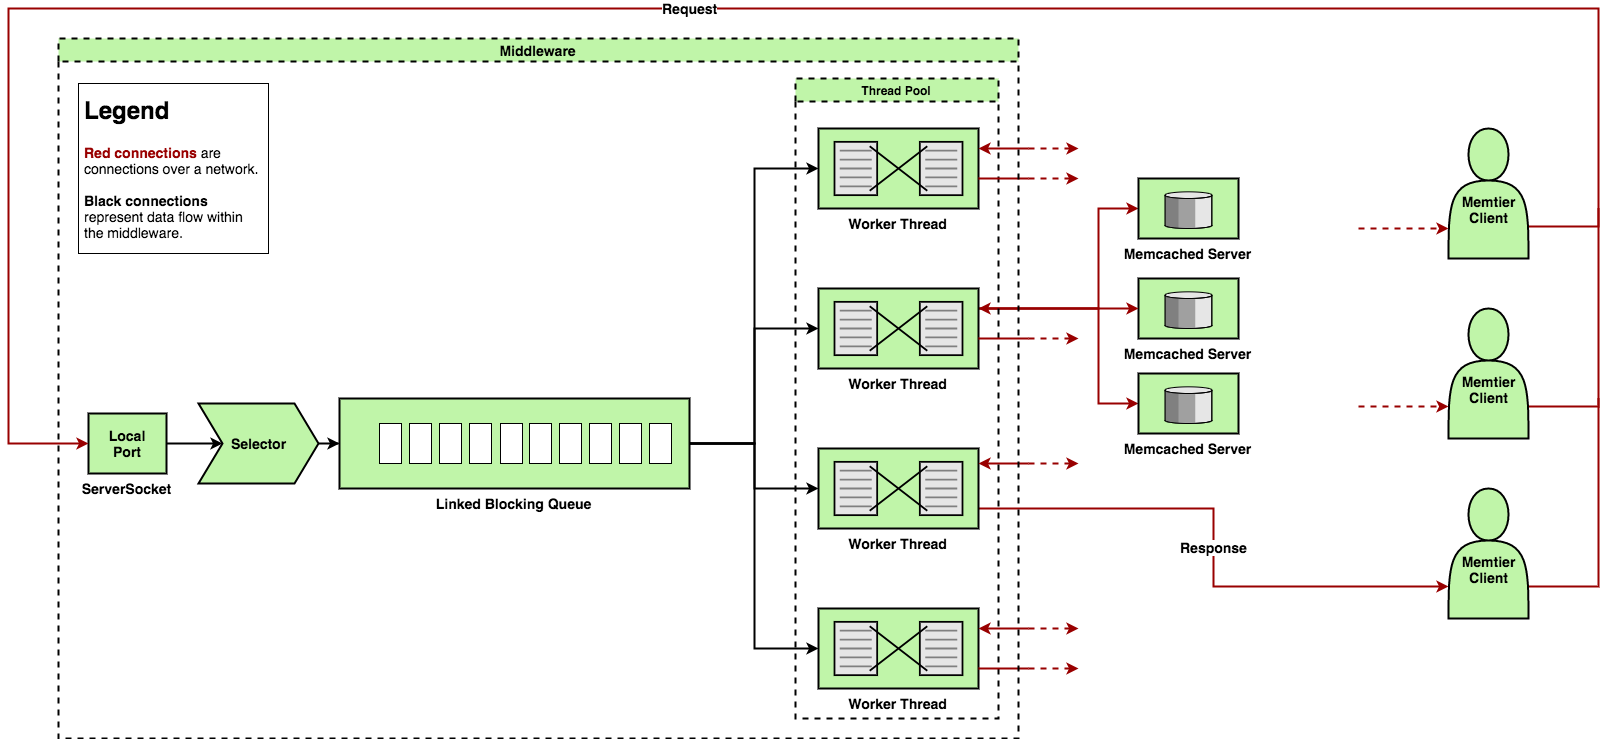
\includegraphics[width=\textwidth]{processing/graphics/system_overview.png}
    \caption{System Overview}
    \label{png::system_overview}
\end{figure}

As can be seen in figure \ref{png::system_overview}, a selector is attached to the server socket in order to accept connections from clients. The key attached to the client connection is then passed with the request such that the workers can communicate the response back to the clients. The reason for the selector is to allow client connections to remain open until explicitly closed by the client. Hence the role of the selector is also to allow new connections and to add them to its internal register of client connections. Once in the internal register (the connection is accepted), the client can send a request which will be read by the net-thread and added to the queue with a reference to the client key. The worker threads then get requests off the queue and process them one by one. The workers first parse the request to get the command type. If the command is invalid, an error message is immediately sent back to the client associated with this request. Otherwise, the worker then communicates with the memcached server(s) in order to store or retrieve data. The servers' response(s) are then parsed again to check for errors and statistics, and a response, potentially merged, is sent to the client.

\subsection{Selector}
The selector serves as a register for connected clients. It is used as passing a socket channel in the queue as part of the request forces the connection to be closed at completion of the request. Hence the selector accepts connections from clients and registers all connected clients. The selector then listens to the registered clients for messages sent to the server socket it is connected to and generates ``read events'' for each client sending messages to the socket. Simultaneously, the net-thread permanently checks for read events generated by the selector and reads data from the client associated with the event to a buffer. This buffer is then added as a request to the queue. Note that the selector key and a timestamp are added to the buffer to form a complete request on the queue. Moreover, note that the use of a selector forces to use non-blocking IO on the client side. However, this is not a problem since any read event guarantees that data can be read from the socket, hence avoiding the use of reading loops.

\subsection{Worker Threads}
A thread pool executor of fixed size is used to organise the worker threads. This has the advantage that it reduces thread environment switching if there is not need for an extra thread to be used. This could be the case when the connection to the memcached servers are extremely fast. In such a case, the executor will not use more threads than are available from the hardware as reusing the same thread to process the next request does not involve any overhead compared to switching to another thread to perform the same work. However, as soon as server service times increase, the thread pool allows to perform work on some thread while another is idle awaiting a response from memcached. Moreover, the thread pool executor has the advantage that if some thread crashed during the execution of the middleware, it will automatically be relaunched. Hence it should in theory provide more stability to the system.

The worker threads perform close to the entirety of the work within the middleware. The reason these workers perform the most work is that the work can be performed concurrently and, ideally, it is performed in parallel. In the initial design, even the reading of the socket was performed by the workers to avoid creating a buffer (containing the message sent from the client) for each request. However, this leads to request duplication as the read event was active as long as nothing was read from the socket, hence repeatedly adding requests to the queue if the initial request had not already been read. This is easily caused by even non-significant queue times. Therefore the design was changed, at the cost of creating a byte buffer for each request.

When launching a thread, two buffers are created. One is used for temporary data while the other contains the response from memcached to be sent back to clients. Note that all buffers used in the middleware are of size 16384 bytes as this allows for 10 keys of size 250 bytes and 10 values of 1024 bytes (and some margin) to be stored in the buffer. The temporary data buffer is mostly used to interpret individual responses from the memcached servers and its data is then added to the buffer containing the aggregate data for the client. Creating only two buffers for each worker has the goal to reduce dead times created by the garbage collector. Exactly how individual request types are handled by the middleware and how the buffers are utilised is explained in a later section.

Each worker is connected to all backend memcached servers at all times. These channels are blocking to ensure that the worker awaits a response from the servers when reading from a channel. Should a worker crash, the thread pool executor will rebuild a thread to replace it and the connections to the servers should be reestablished. However, note that such a situation never occurred during testing.

\subsection{Requests}
All requests are built from the following:
\begin{itemize}
    \item A buffer containing the data sent from the client. This is known when the request object is created.
    \item A selection key that refers to the client who sent the request. This is used to recover the channel to said client in order to sent him the response. Note this has nothing to do with the memcached key used to refer to the data stored on the backend servers.
    \item A type which can be either:
    \begin{enumerate}
        \item GET: a simple get request with a single key.
        \item SET: a simple set request with one key and the data to be set as the value for that key.
        \item MULTIGET: a get request with more than one key.
        \item INVALID: a request that does not conform to the protocol defining the format of the three commands above.
    \end{enumerate}
    This is not known when the request is created and will only be known once a worker parses the request.
    \item A boolean identifying the request as a hit. Note that the notion of hit is different for each type of request. In the case of a \mintinline{java}{get}, it simply identifies whether a value was returned by the memcached servers. In the case of a \mintinline{java}{set}, this represents whether a server responded with something different to \mintinline{java}{STORED}. In the cases of \mintinline{java}{multiget} and \mintinline{java}{invalid} request, this boolean does not have any meaning. \mintinline{java}{multiget} hits are handled directly as the responses from memcached are parsed.
    \item Several timestamps:
    \begin{enumerate}
        \item The time the request is created. This is (obviously) known when the request is created.
        \item The time the request is dequeued. The worker updates this timestamp as soon as the request is taken from the queue.
        \item The time the request was transmitted to the servers. This timestamp is taken just before any messages are sent to memcached.
        \item The time memcached answered. This is taken once \textit{all} memcached servers that were contacted for this request have answered.
        \item The time the request was completed. This is the timestamp taken when the complete response was sent back to the client.
    \end{enumerate}
\end{itemize}

All requests are parsed only at the worker level, hence the majority of the fields defined above are only known once the request is being processed by some worker.

When parsing a request, the first aspect that is checked is whether the request terminates with \mintinline{java}{"\r\n"}. Then the command is parsed up to the first occurrence of \mintinline{java}{"\r\n"}. The set of bytes preceding these two characters is converted to a string and the first word in said string is compared to known command words (i.e. \mintinline{java}{get} or \mintinline{java}{set}). Once it is established which type the command is, the rest of the command is checked for correctness. In the case of \mintinline{java}{get}, the number of arguments is checked in order to determine whether the command should be treated as a \mintinline{java}{multiget}. In the case of a \mintinline{java}{set}, it is checked if the data block attacked to the request is of the length specified in the command. If any of these tests fail, the command is flagged as invalid and an error string is sent back to the client. In this case there is no communication with the backend memcached servers as the request does not conform to the protocol.

\subsubsection{Sets}
Once a command has been dequeued, parsed, and established as type \mintinline{java}{set}, all worker buffers are cleared and the original request buffer is transmitted to all backend servers. The worker thread then awaits responses from the servers in the same order as he sent out the request. As we use blocking input/output on the server side, the same order is chosen as the first contacted server is likely the first to respond. Note however that if the connection to the first memcached server is significantly slower than other connections, this will result in inefficient time utilisation as the middleware will wait for this response first, even though the responses from other servers might already be available. Every response is then checked and if anything other than \mintinline{java}{"STORED\r\n"} is returned from any server, that response is returned to the client and the \mintinline{java}{set} is flagged as a miss. The rest of the servers' responses are read in order to make sure all communication channels are cleared for the next request.
\begin{figure}[h]
    \centering
    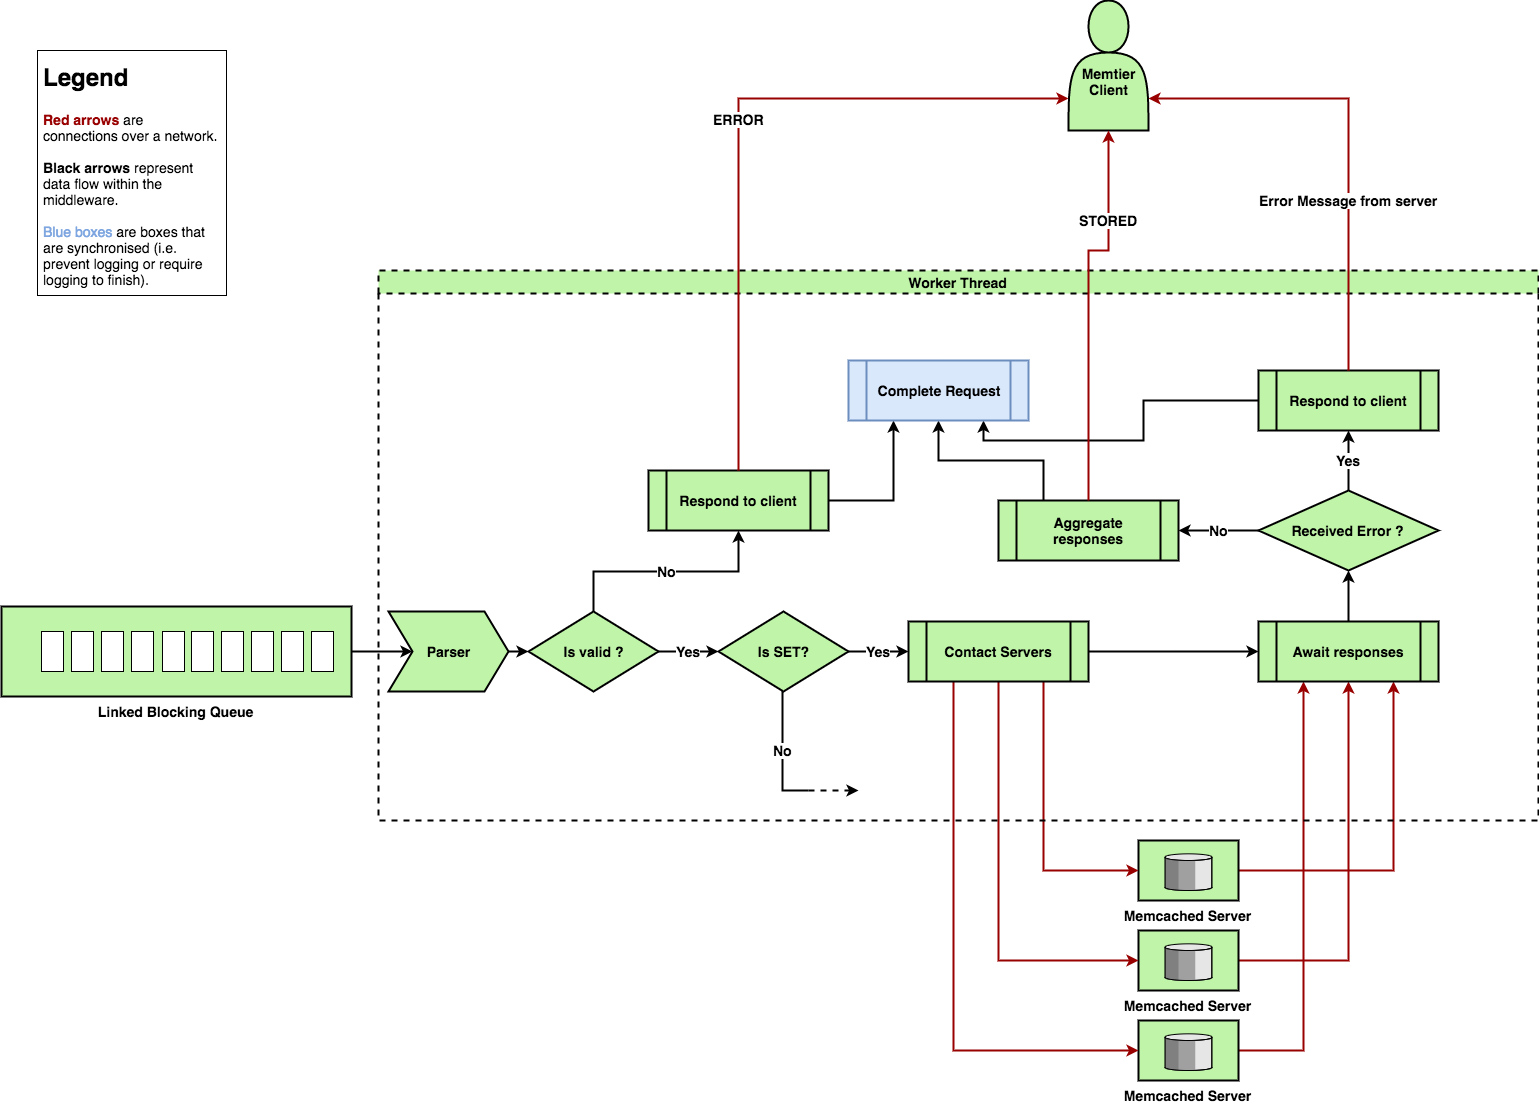
\includegraphics[width=\textwidth]{processing/graphics/sets_handling.png}
    \caption{Handling of \mintinline{java}{SET} requests}
    \label{png::sets_handling}
\end{figure}
In the case of a hit (i.e. all servers responded \mintinline{java}{"STORED\r\n"}), this is relayed to the client and the request is completed. Request completion will be described under logging and thread synchronisation below.

Note that that during the time the request is handled, the appropriate timestamps are updated for the request.

\subsubsection{Gets and Non-Sharded Multigets}
As these requests are not sent to all memcached servers, load balancing is in order. To perform load balancing, a server is chosen by simply taking the least recently used server across all workers. Of course, this can be suboptimal if the least recently used server is still working on a large request and other servers have already freed after handling smaller requests. However, due to relatively strong variations in the network latencies, it is very difficult to predict the time needed for a server to process a request.

\begin{figure}[h]
    \centering
    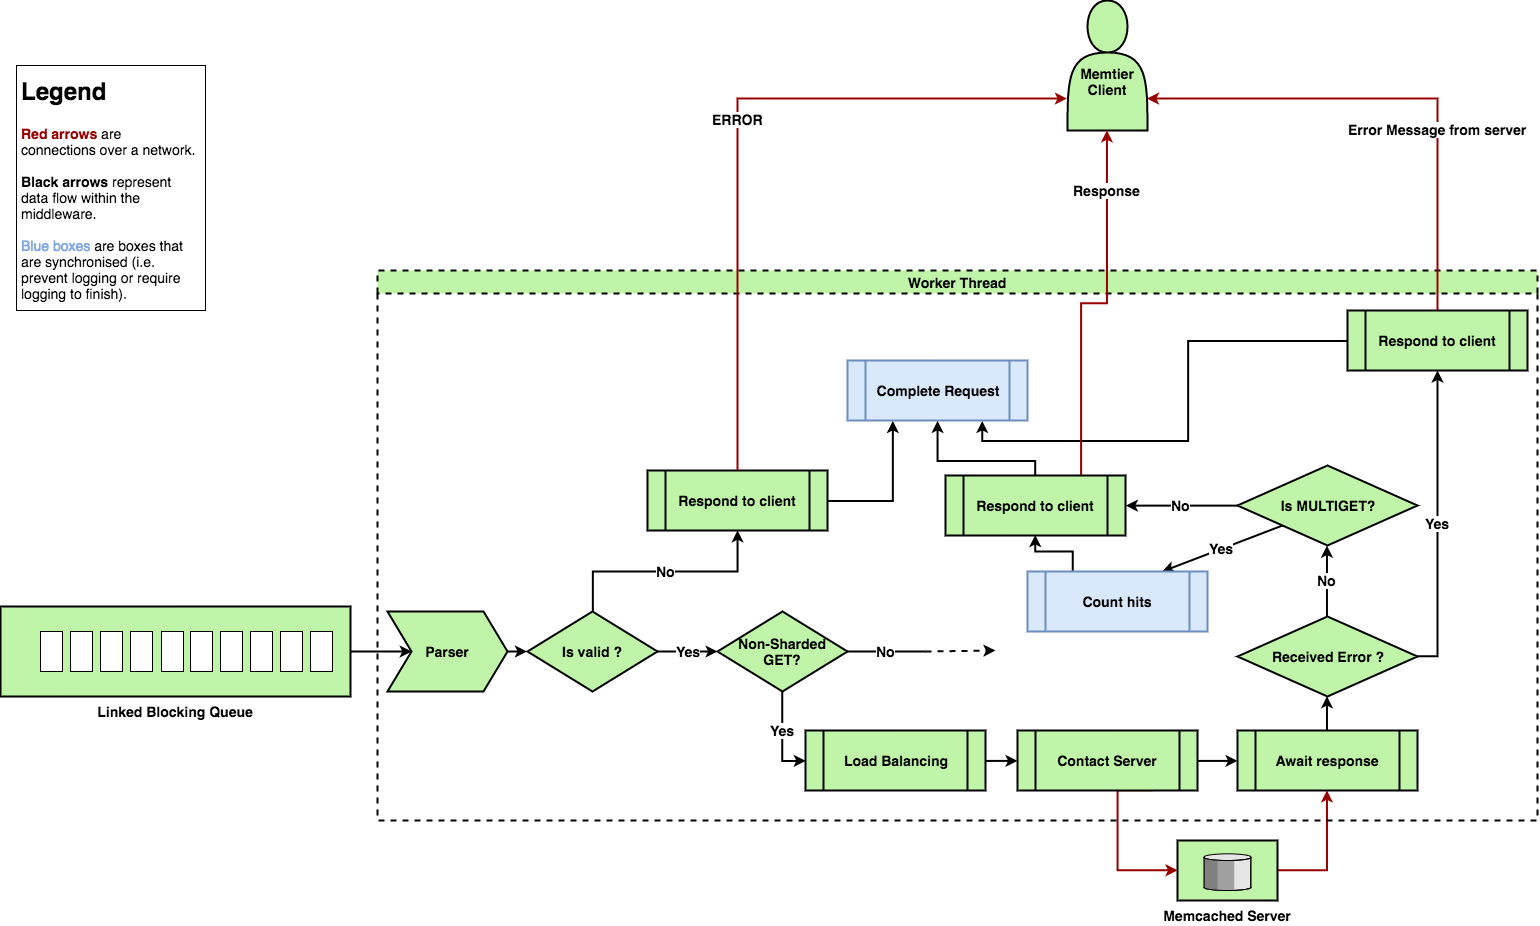
\includegraphics[width=\textwidth]{processing/graphics/gets_handling.png}
    \caption{Handling of \mintinline{java}{GET} and non-sharded \mintinline{java}{MULTIGET} requests}
    \label{png::gets_handling}
\end{figure}

The request, as it was received by the client, is then sent to the selected server. The worker awaits a answer and continuously reads from the channel until the response either ends with \mintinline{java}{"ERROR\r\n"} or matches an error (anything ending with \mintinline{java}{"ERROR\r\n"}, i.e. also \mintinline{java}{"SERVER_ERROR\r\n"} or \mintinline{java}{"CLIENT_ERROR\r\n"}). Note that this does not create a hot loop as the channel reading is blocking.

If the request is of type multiget, the worker checks how many values were included in the response compared to the number of values requested in the command. This then determined the number of hits and misses of the request.

For a get, the response is compared to \mintinline{java}{"END\r\n"} and checked if it ends with \mintinline{java}{"ERROR\r\n"}. If neither is the case, the request is flagged as a hit.

Both for \mintinline{java}{multigets} and single \mintinline{java}{get}, the response is then relayed to the client and the request completed.


\subsubsection{Sharded Multigets}
In the case of a sharded multigets, the \mintinline{java}{readSharded(request, response_buffer, temp_buffer)} function is called. This function completely takes care of the handling of such requests with the exception of request completion. Sharded requests are handled in two ways (graphically shown in figure \ref{png::multigets_handling}):
\begin{enumerate}
    \item If the number of requested values is less than the number of available memcached servers, load balancing is performed and a single \mintinline{java}{get} is sent to a server. Again, the servers responses are interpreted in the same order as the servers were contacted. If an error is received from any server, \mintinline{java}{"ERROR\r\n"} is relayed to the client and the server channels are cleared for the next request. Otherwise individual responses are read into the temporary buffer, \mintinline{java}{"END\r\n"} is removed from the end of the buffer and the entire buffer is appended to the response buffer.
    \item If the number of request values is larger than the number of available memcached servers, no load balancing is required as all servers will need to be contacted anyways. The processing is then performed as above.
\end{enumerate}
\begin{figure}[h]
    \centering
    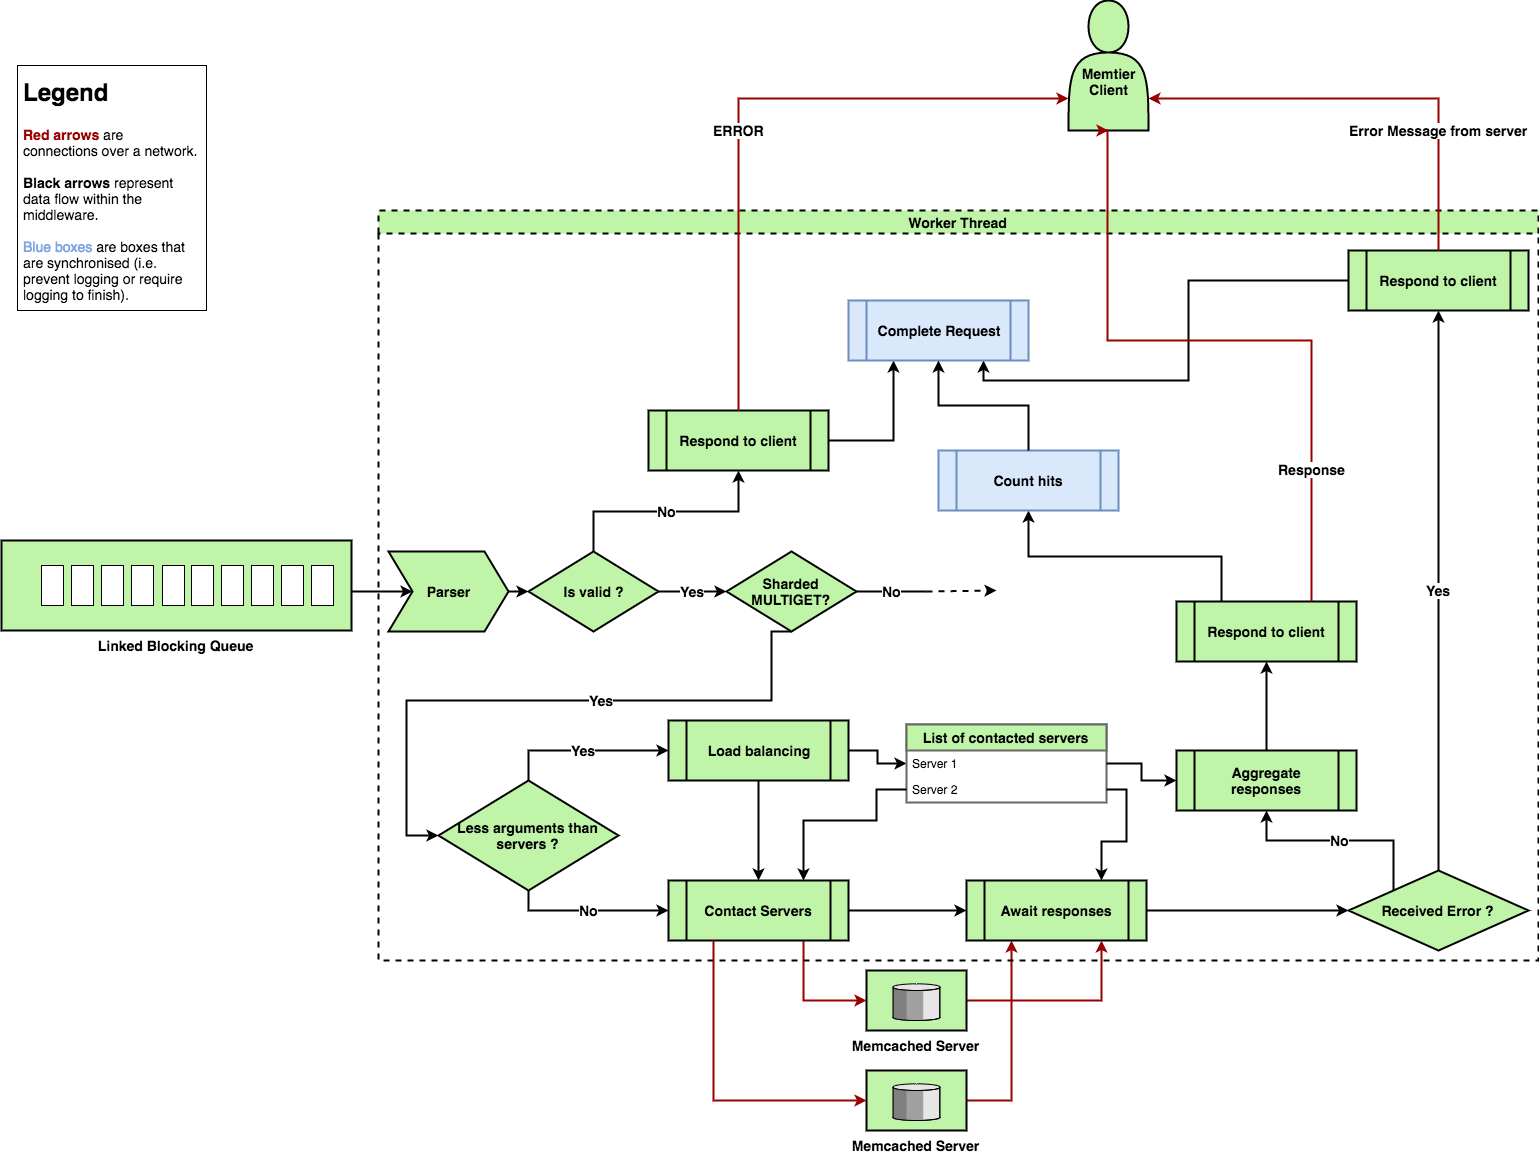
\includegraphics[width=\textwidth]{processing/graphics/multigets_handling.png}
    \caption{Handling of sharded \mintinline{java}{MULTIGET} requests}
    \label{png::multigets_handling}
\end{figure}
When all memcached servers have answered, \mintinline{java}{"END\r\n"} is added to the response buffer and the response is relayed to the client unless an error occurred in one of the servers. The response buffer is then converted into a string to check the number of hits. Note that this is performed irrespective of a server responding \mintinline{java}{"ERROR\r\n"}.


\subsection{Logging, Request Completion and Thread Synchronisation}
All statistical data relating to a request is stored within the request itself. Hence the reserved fields for timestamps, type and hit flags. When a request is completed, the \mintinline{java}{complete(request)} private method of that worker object is called. This method is then computes the required statistics and stores them internally in the corresponding worker object. Hence note that up until the completion of the request, no internal data of the worker was touched with the exception of \mintinline{java}{multigets} hit counting.

Every part of the workers that accessed internal statistics data is synchronised with respect to the worker object. Hence both the \mintinline{java}{complete(request)} and the \mintinline{java}{multiget} hit counting are synchronised. This ensures memory data consistency when accessing the internal statistical data for logging. Hence all data should be consistent and no request should only partially logged unless the logger kicks in between two boxes in figures \ref{png::gets_handling} and \ref{png::multigets_handling}. This can only happen during the handling of multigets and creates hits to be registered even though the request is incomplete. This is very unlikely to happen as close to no work is performed between any two blue boxes. Moreover, note that this does not affect any final statistics.

The logging is performed by a static function:
\begin{minted}{java}
    public static String getRecord(ArrayList<Worker> workers, int queueLength);
\end{minted}
(of the worker class) that, when accessing the internal data of a worker in its argument list, locks that worker, hence preventing it from modifying its internal statistical data. This is done in order to get consistent interval information when logging. \\
Every second, the \mintinline{java}{getRecord()} function is called on all workers and gathers their statistical data to output what has happened in the last second. Note that this does not prevent the worker from performing work until it reaches either request completion or a multiget hit count update. Due to the fact that data gathering is relatively fast compared to the overall time needed to process a request and the server time, this usually does not affect performance. Moreover, note that not all workers are blocked but only the one currently being accessed. This can create slightly offset data when the middleware is launched with a large number of workers as the last few workers might complete some requests while the data from the first worker is being read. However, this only affects the time interval, not the overall data, because the logger only gathers data from since \mintinline{java}{getRecord()} was called \textit{on that worker}. Hence, even if the last worker completes more requests while the data from the first worker is being collected, these completed requests will not be considered the next time \mintinline{java}{getRecord()} is called on that worker.

Furthermore, \mintinline{java}{getRecord()} also takes care of clearing any histogram information stored in workers when running for the first time. This is to ensure that histogram data does not include requests completed during warm up time. The warm up time is set to ten seconds, therefore \mintinline{java}{getRecord()} is called ten seconds after the launch of the middleware and then again every second after that.

The analysis data is logged both to console and to an \mintinline{shell}{analysis.log} file in the home directory. Note that the logs in the log file additionally contain timestamps. Moreover, the middleware logs system information such as interruptions, errors settings up sockets, connection request, etc. to \mintinline{shell}{system_report.log} also in the home directory.

On top of that, when the \mintinline{java}{ShutdownHook} is triggered, statistics for individual workers is gathered and the histogram is printed. The statistic for individual workers include queue time, processing time, server time, total count, hits per second and misses per second for each request type. The final statistics layout is very similar to the one provided my memtier.

\subsection{Terminology}
This section describes the terminology used across all experiments unless explicitly specified otherwise.
\begin{description}
    \item[Response time/latency as given by middleware]\hfill\\ This refers to the time between creation of a request when read from the server socket to the time the request is completed (i.e. the response has been sent to the client). Thus this does not include the time the request and response spend in the network between the client and middleware hosts.
    \item[Processing time]\hfill\\ This refers to \textit{all} time between the moment a request is dequeued and the moment the request is completed. Hence this fully includes server time.
    \item[Server time]\hfill\\ Server time refers to the time between the moment a request is forwarded to \textit{any} memcached server and the time a response has been received from \textit{all} necessary memcached server. Hence in the case of sharded multigets and sets, it is measured from just before the first server is contacted to just after the last response is received. Note that this also includes network latencies between middleware and servers.
    \item[Standard deviation]\hfill\\ Unless explicitly stated otherwise, the standard deviation is the deviation between the average \textit{interval} measurements of some specific software. These intervals are always one second in length. Hence the standard deviation of the latencies measured by 2 clients is the deviation of the results obtained from taking, each second, the average latency measured by both clients. The purpose of this is to show the deviation of the overall system from it's mean behaviour over the experiment time window.
    \item[Server]\hfill\\ A machine running an instance of memcached.
\end{description}

\subsection{Overall Experimental Design}
All repetitions taken are at least 90 seconds long. The ten first seconds are evicted (warm up time) and the 80 next measurements are taken as the data. For client and server data, only the first eight seconds are evicted as the automation scripts allow two seconds for the middleware to boot properly before launching the clients. Note that due to \mintinline{java}{ssh} network latencies, the 80 second windows of measurements might not perfectly coincide between clients, middleware, and servers, but this should be insignificant compared to the overall length of a repetition. The effect of this can be seen in the slight differences of throughput between client and middleware data. However, as will be shown in the first middleware baseline, this is an irrelevant difference.

The error bars used for all graphs are obtained from the standard deviation as described in the terminology subsection above. Deviation of the averages across repetitions are also available in the final data sheets (\mintinline{shell}{/processing/final/<experiment_name>/data.csv}) but will not be used unless relevant. This would be the case if one repetition is deviating from the average significantly.






\newpage

\section{Baseline without Middleware}
The experiments under this section are performed without a middleware. The purpose of this is to establish some benchmark to determine the behaviour of memtier and memcached. For both read-only and write-only workloads, client ranges from two to 56 \textit{per thread} were chosen. In the first experiment, a single memcached machine was connected to three client machines all running two threads.\\
In the second experiment, a single client machine running two instances of memtier was attached to two server machines. Both instances of memtier ran on a single thread.

\subsection{One Server}
This experiment deals with the performance of memcached. Three client machines running memtier with two threads each are connected to a single memcached machine. Figure \ref{png::bench_memcached_through-clients} shows the throughput of read-only and write-only requests with respect to the total number of clients.

\begin{figure}[!h]
    \centering
    \begin{minipage}[b]{.45\textwidth}
        \centering
        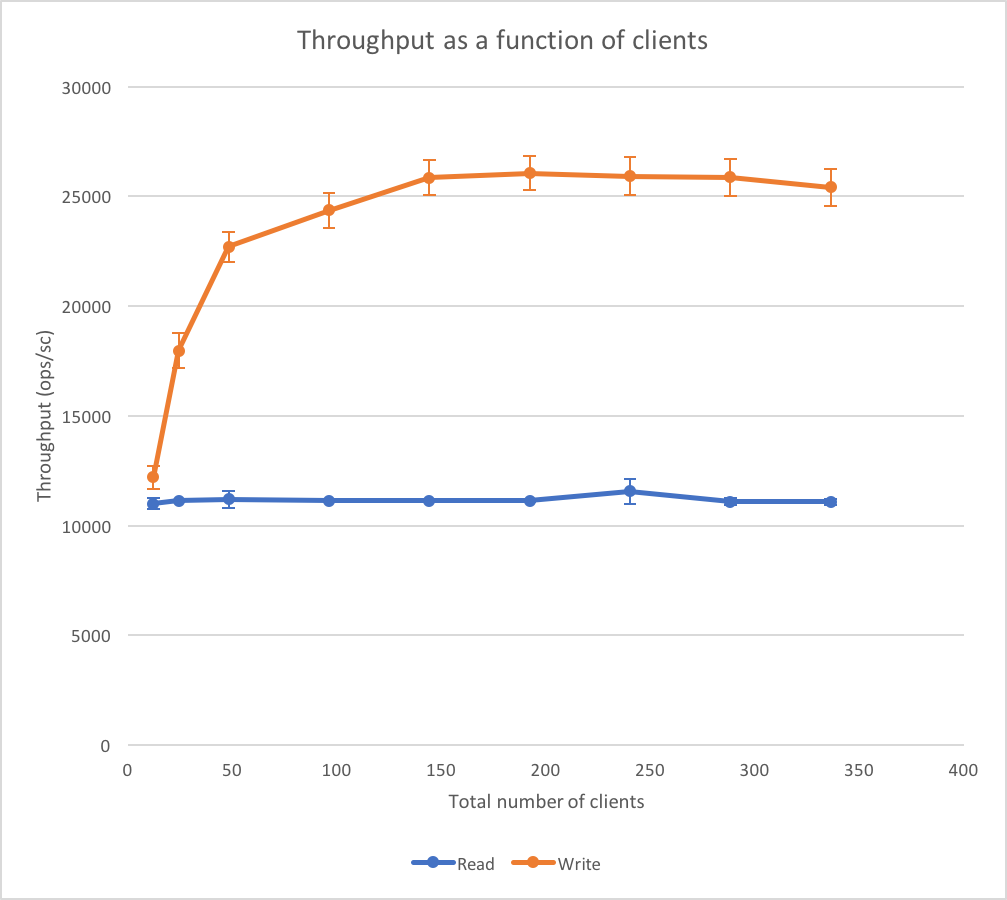
\includegraphics[width=\textwidth]{processing/graphics/bench_memcached_through-clients.png}
        \caption{Throughput as a function of total number of clients}
        \label{png::bench_memcached_through-clients}
    \end{minipage}
    \qquad
    \begin{minipage}[b]{.45\textwidth}
        \centering
        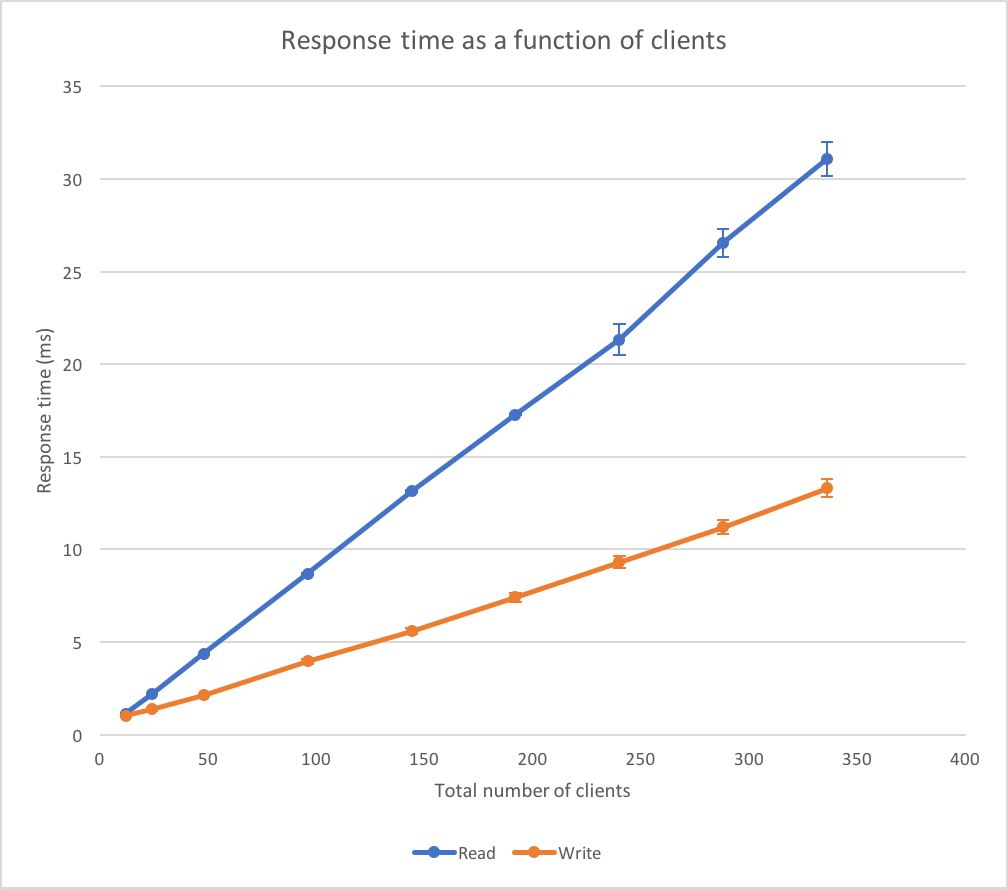
\includegraphics[width=\textwidth]{processing/graphics/bench_memcached_latency-clients.png}
        \caption{Response time as a function of total number of clients}
        \label{png::bench_memcached_latency-clients}
    \end{minipage}
\end{figure}

Figure \ref{png::bench_memcached_latency-clients} shows the respective response time with respect to total number of clients.



\subsubsection{Explanation\label{section::computation_reads}}
First note that the experiment obeys the interactive law. This can be seen in figure \ref{png::bench_memcached_inter_law}. The response time logged by the clients coincides perfectly with the response time computed by the interactive law. Note that graphs illustrating the interactive law will not be shown in later experiments unless the measurements used to graph throughput and response time do not obey operational laws.
\begin{figure}[!h]
    \centering
    \begin{minipage}[b]{.45\textwidth}
        \centering
        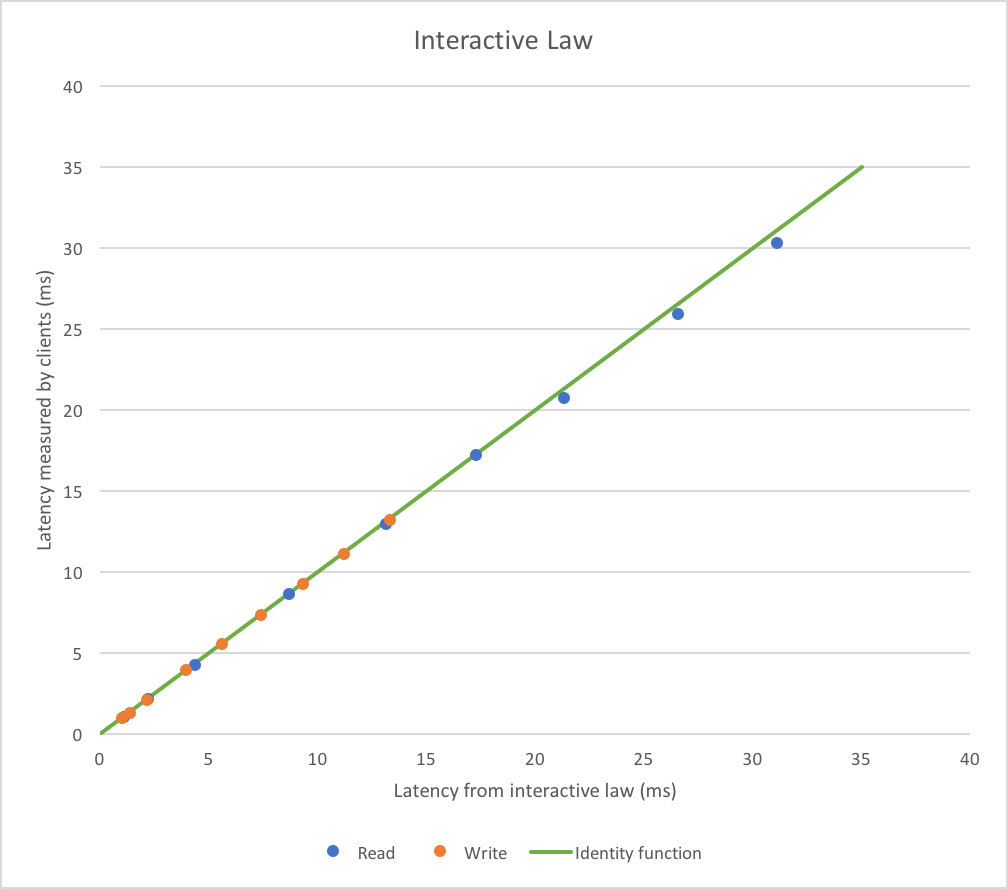
\includegraphics[width=\textwidth]{processing/graphics/bench_memcached_inter_law.png}
        \caption{Latency measured by clients versus interactive law latency}
        \label{png::bench_memcached_inter_law}
    \end{minipage}
    \qquad
    \begin{minipage}[b]{.45\textwidth}
        \centering
        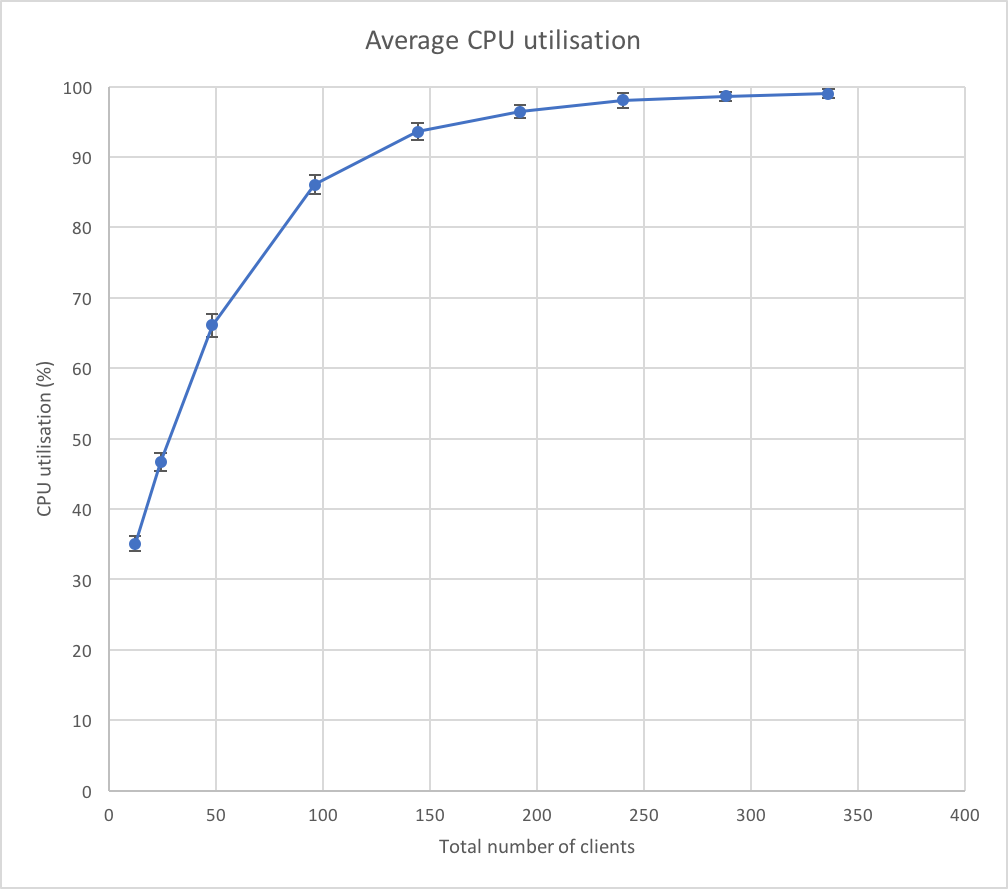
\includegraphics[width=\textwidth]{processing/graphics/bench_memcached_cpu_util.png}
        \caption{Average CPU utilisation based on total client count}
        \label{png::bench_memcached_cpu_util}
    \end{minipage}
\end{figure}

First consider write throughput. Memcached seems to attain saturation at around 150 clients as shown in figure \ref{png::bench_memcached_through-clients}. Figure \ref{png::bench_memcached_cpu_util} indicates that the saturation level is reached due to CPU utilisation.\\
Second, for read throughput, saturation is already reached with 12 clients total. This is due to network bandwidth. \mintinline{java}{dstat} data indicates that the average network upload of memcached is 12 megabytes per second. From \mintinline{java}{iperf}, we know that the server upload bandwidth is also 12 megabytes per second ($96.4\text{Mbps}/8=12.05\text{MBps}$\footnote{\label{source::server_net}\mintinline{shell}{/logs/server1_netowork.log}}). Hence memcached cannot handle more than around 11 thousand requests per second. Note that this number makes sense since only hits occurred and data blocks are of size 1024 bytes. Then we have $11.000 \times 1024 = 11 264 000$ bytes of data uploaded to the network by the server. Note that this does not include any keys, \mintinline{java}{VALUE} and \mintinline{java}{END} statements, hence the number being slightly lower than the average network upload bandwidth measured by \mintinline{java}{iperf}.


\subsection{Two Servers}
This experiment has the goal to check for saturation levels of client machines. Figures \ref{png::bench_clients_through-clients} and \ref{png::bench_clients_latency-clients} show throughput and latency as a function of the total number of clients respectively. Note that in this case, there is no significant difference in behaviour between read-only and write-only workloads. Still the interactive law hold as shown in figure \ref{png::bench_clients_inter_law}. Note that on low ranges of latencies, the response time measured by the clients is higher than the one computed by the interactive law. This is due to the fact that response times observed at low loads vary greatly between memtier instances on the same machine\footnote{\mintinline{shell}{/processing/processed/benchmark_clients/**/clients.csv}}. This is likely caused by different network latencies between the client machine and the two server machines.
\begin{figure}[!h]
    \centering
    \begin{minipage}[b]{.45\textwidth}
        \centering
        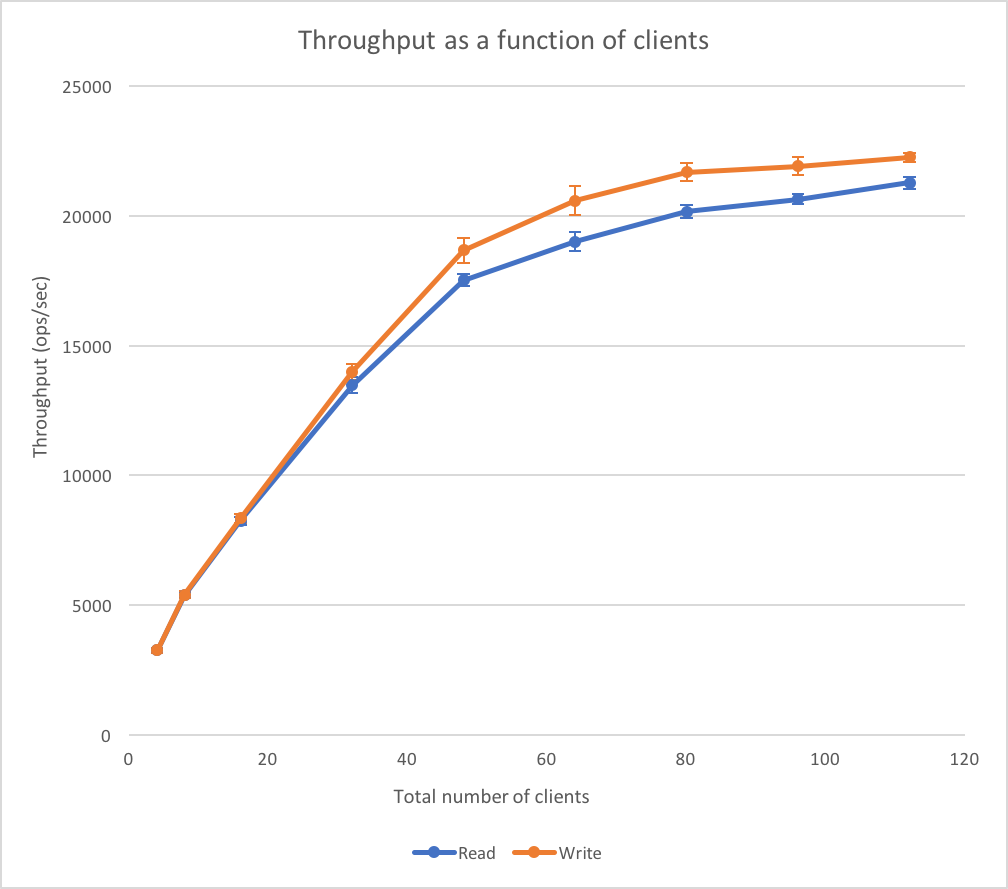
\includegraphics[width=\textwidth]{processing/graphics/bench_clients_through-clients.png}
        \caption{Throughput as a function of total number of clients}
        \label{png::bench_clients_through-clients}
    \end{minipage}
    \qquad
    \begin{minipage}[b]{.45\textwidth}
        \centering
        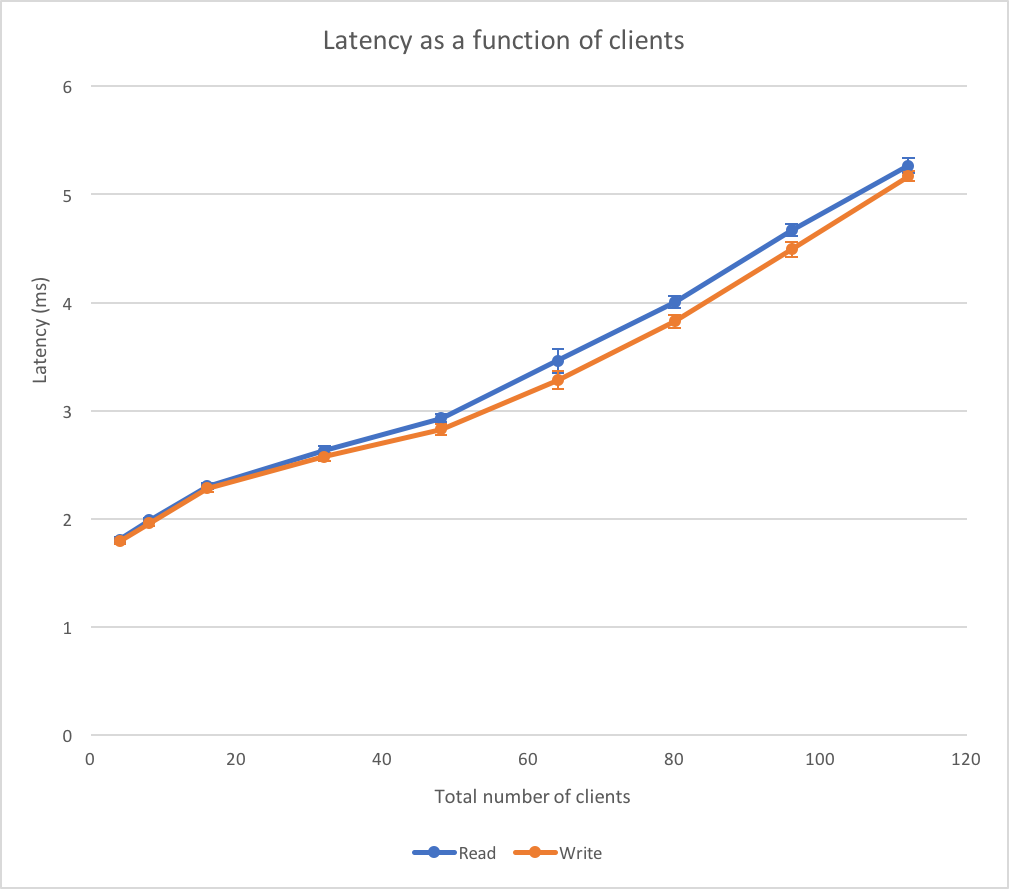
\includegraphics[width=\textwidth]{processing/graphics/bench_clients_latency-clients.png}
        \caption{Response time as a function of total number of clients}
        \label{png::bench_clients_latency-clients}
    \end{minipage}
\end{figure}

\subsubsection{Explanation}
For both reads and writes, the memtier instance connected to the first server attains maximum throughput at 24 clients per thread\footnote{\mintinline{shell}{/processing/processed/**/clients_24/clients.csv}}. However, the memtier instance connected to the second instance only attains maximum throughput at 48 to 56 clients per thread\footnote{\mintinline{shell}{/processing/processed/**/clients_48/clients.csv}}. This causes the dent in figure \ref{png::bench_clients_latency-clients} at 48 total clients. Beyond that point, the latency for the first instance of memtier starts to increase much more due to saturation hence dragging the average upwards. Thus, optimally, the first instance would run with 24 clients and the second one with 48 or 56 clients to achieve maximum throughput. As only configurations with the same number of clients across all memtier threads are considered, the maximum throughput is chosen at a workload of 80 total clients for reads and for writes (40 clients per thread).

For any operation, the bottleneck is the network. Figures \ref{png::bench_clients_net_reads} and \ref{png::bench_clients_net_writes} show the data written to network per second for reads and writes respectively. Note that for all graphs, averages are taken across machines. Therefore, the data written to network per second given by the blue line in figures \ref{png::bench_clients_net_reads} and \ref{png::bench_clients_net_writes} is the average \textit{per server}.

\begin{figure}[!h]
    \centering
    \begin{minipage}[b]{.45\textwidth}
        \centering
        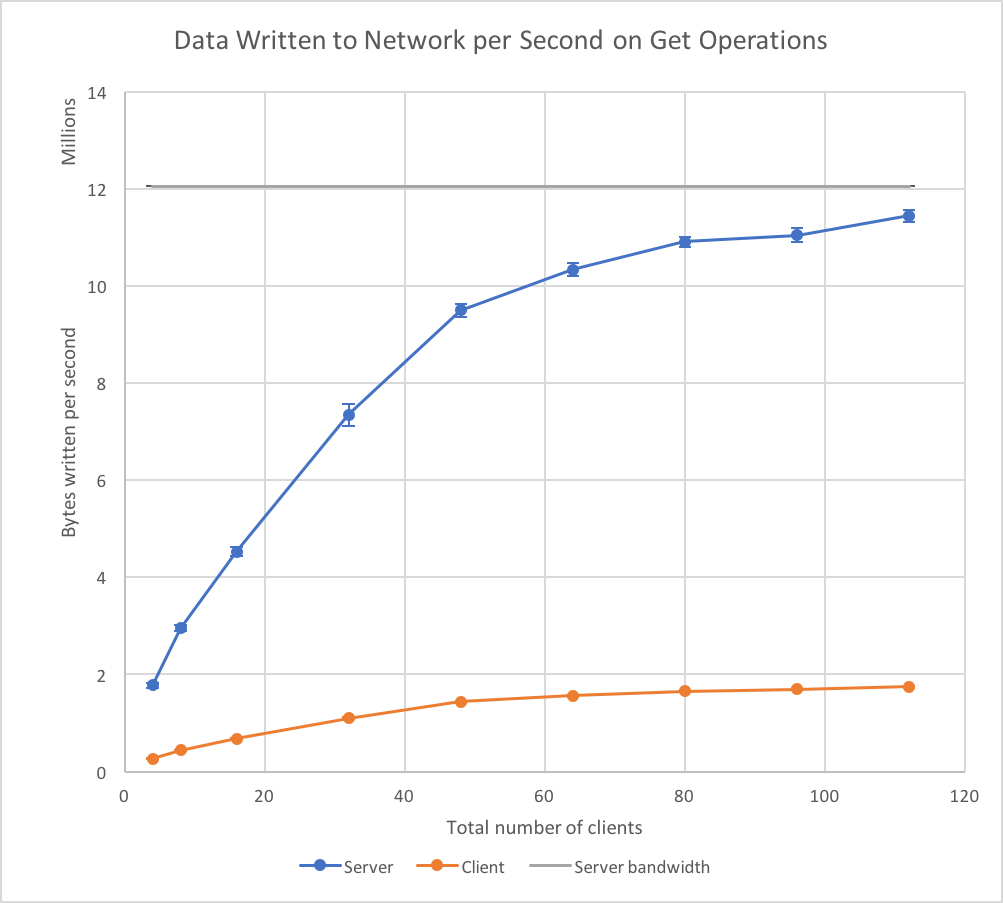
\includegraphics[width=\textwidth]{processing/graphics/bench_clients_net_reads.png}
        \caption{Data written to network per second on reads}
        \label{png::bench_clients_net_reads}
    \end{minipage}
    \qquad
    \begin{minipage}[b]{.45\textwidth}
        \centering
        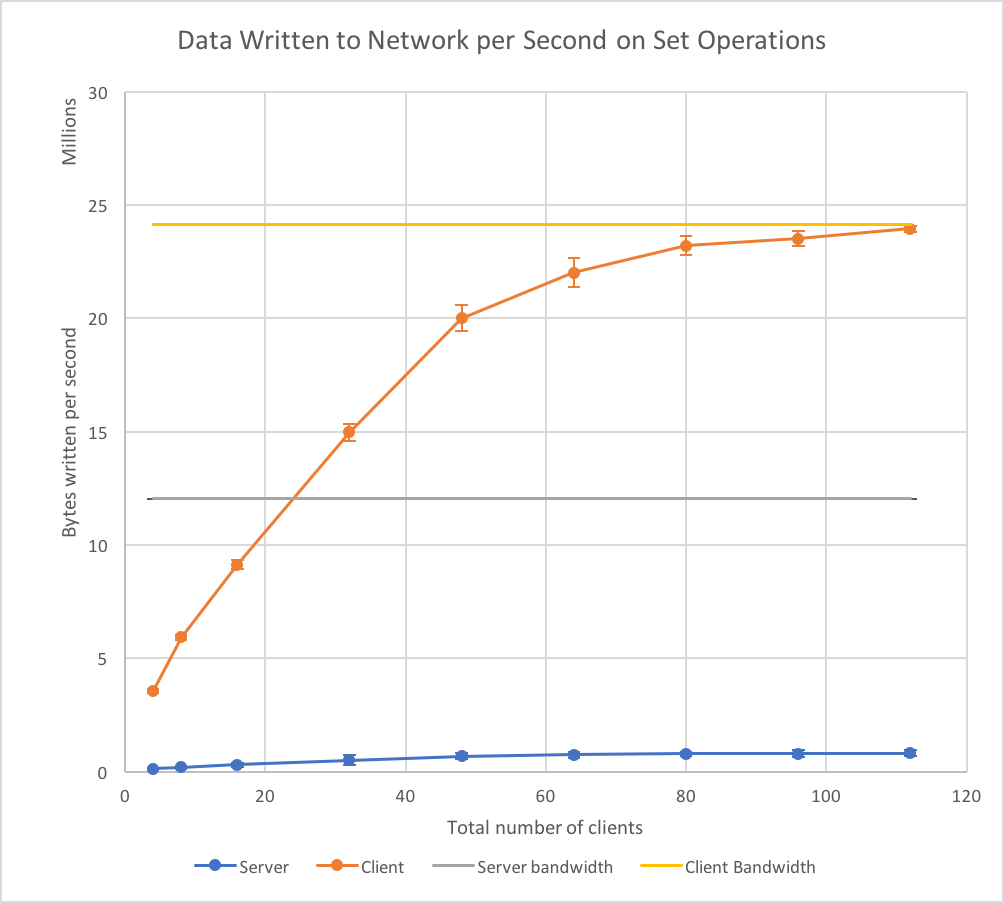
\includegraphics[width=\textwidth]{processing/graphics/bench_clients_net_writes.png}
        \caption{Data written to network per second on writes}
        \label{png::bench_clients_net_writes}
    \end{minipage}
    \begin{minipage}[b]{.45\textwidth}
        \vspace{1cm}
        \centering
        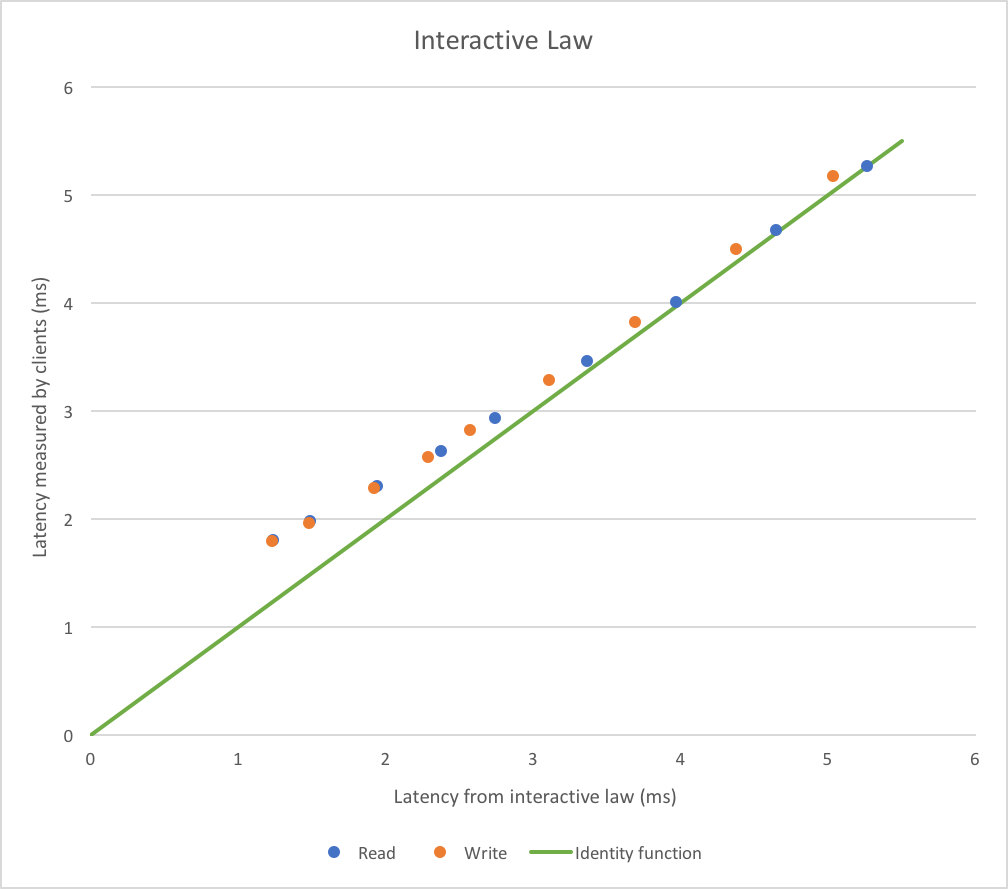
\includegraphics[width=\textwidth]{processing/graphics/bench_clients_inter_law.png}
        \caption{Latency measured by clients versus interactive law latency}
        \label{png::bench_clients_inter_law}
    \end{minipage}
\end{figure}

In the case of reads (depicted in figure \ref{png::bench_clients_net_reads}), one can see that the average data sent over the network per server approaches the bandwidth limit (12.05MB per second\footref{source::server_net}). This is the same situation as in the previous experiment.\\
In the case of writes, the maximum bandwidth for client uploads is 24.125 megabytes per second ($193\text{Mbps}/8=24.125\text{MBps}$\footnote{\mintinline{shell}{/logs/client1_netowork.log}}). Figure \ref{png::bench_clients_net_writes} shows that this is reached relatively fast.

In conclusion, the overall bottleneck in this experiment is the network. For both reads and writes, the network does not allow the machines to reach saturation due to compute power.

\subsection{Summary}
In both experiments, writes generally allow to reach higher maximal throughputs (and hence lower latencies). Generally, running around 70 to 80 clients per client machines also allows to reach the highest throughput without over-saturation and increased latencies due to network bandwidth limits or server compute power bounds. The only exception to this rule is read-only workloads on a single server. In that case, the network bandwidth limit is already reached with much lower client numbers.

The numbers below give the maximum measured throughputs, irrespective of when this is obtained. In the best scenario, the client number with a single server is around 150 total clients. This provides throughput very close to the numbers shown in table \ref{table::max_through_section_2} but with lower response times. Similarly, for one load generating virtual machine, around 70 to 80 clients generate enough load to achieve numbers close to the ones displayed in table \ref{table::max_through_section_2} but with lower response times than with the configuration given in the table.

\begin{figure}
    \centering
    \begin{tabular}{|l|p{2cm}|p{2cm}|p{4cm}|}
        \hline                        & Read-only workload & Write-only workload & Configuration gives max. throughput \\
        \hline One memcached server   &             11 558 &              26 056 &             Write-only; 200 clients \\
        \hline One load generating VM &             21 283 &              22 264 &             Write-only; 112 clients \\
        \hline
    \end{tabular}
    \caption{Maximum throughput of different VMs}
    \label{table::max_through_section_2}
\end{figure}



\newpage

\section{Baseline with Middleware}
In this set of experiments, one load generating virtual machine and one memcached server are used. In the first experiment, a single middleware is used as intermediary between clients and the memcached server. During the second experiment, the client virtual machine is connected to two middleware machines, each getting requests from a single thread memtier instance. Both middlewares then use the same memcached server as backend.

\subsection{One Middleware}
\subsubsection{Reads}
Firstly, figures \ref{png::bench_1mw_through-clients_read_cdat} and \ref{png::bench_1mw_through-clients_read_mdat} show that there is close to no mismatch between throughput data gathered from the client and from the middleware for read operations. The small differences in throughput are caused by the fact that the measurement windows might not coincide perfectly.

\begin{figure}[!h]
    \centering
    \begin{minipage}[b]{.45\textwidth}
        \centering
        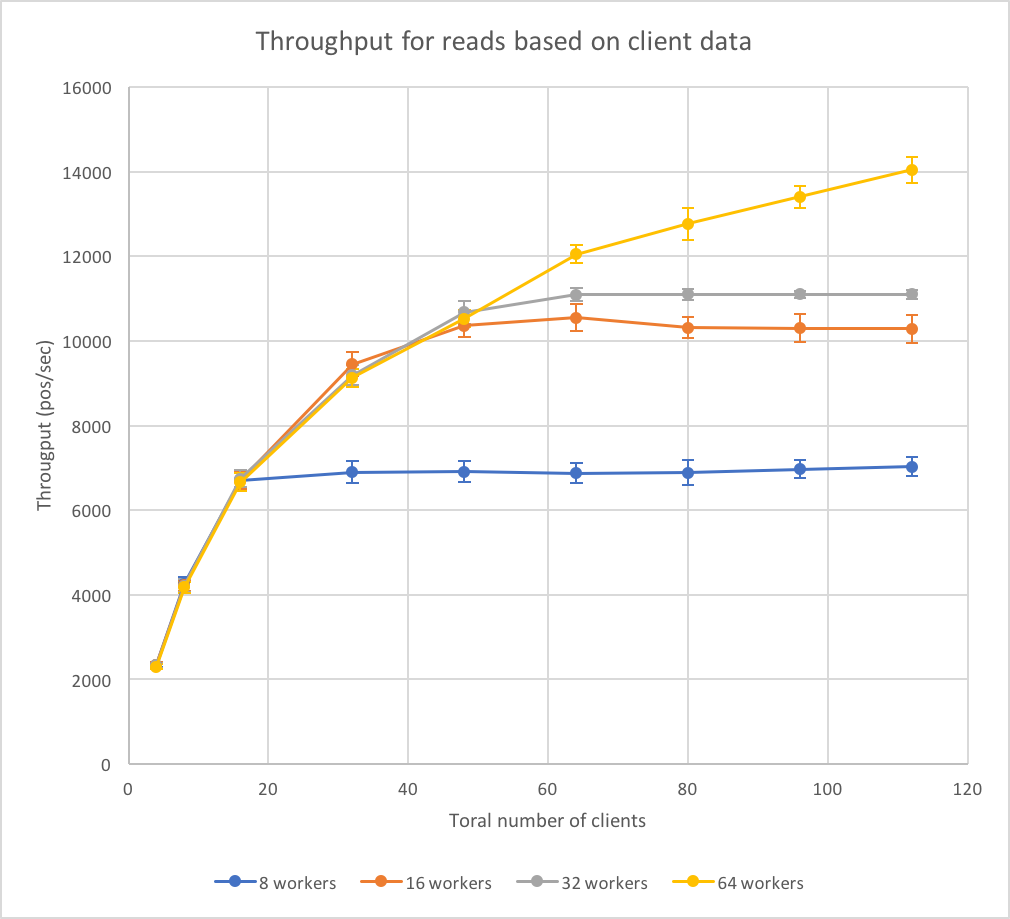
\includegraphics[width=\textwidth]{processing/graphics/bench_1mw_through-clients_read_cdat.png}
        \caption{Throughput as measured by the client machine for reads}
        \label{png::bench_1mw_through-clients_read_cdat}
    \end{minipage}
    \qquad
    \begin{minipage}[b]{.45\textwidth}
        \centering
        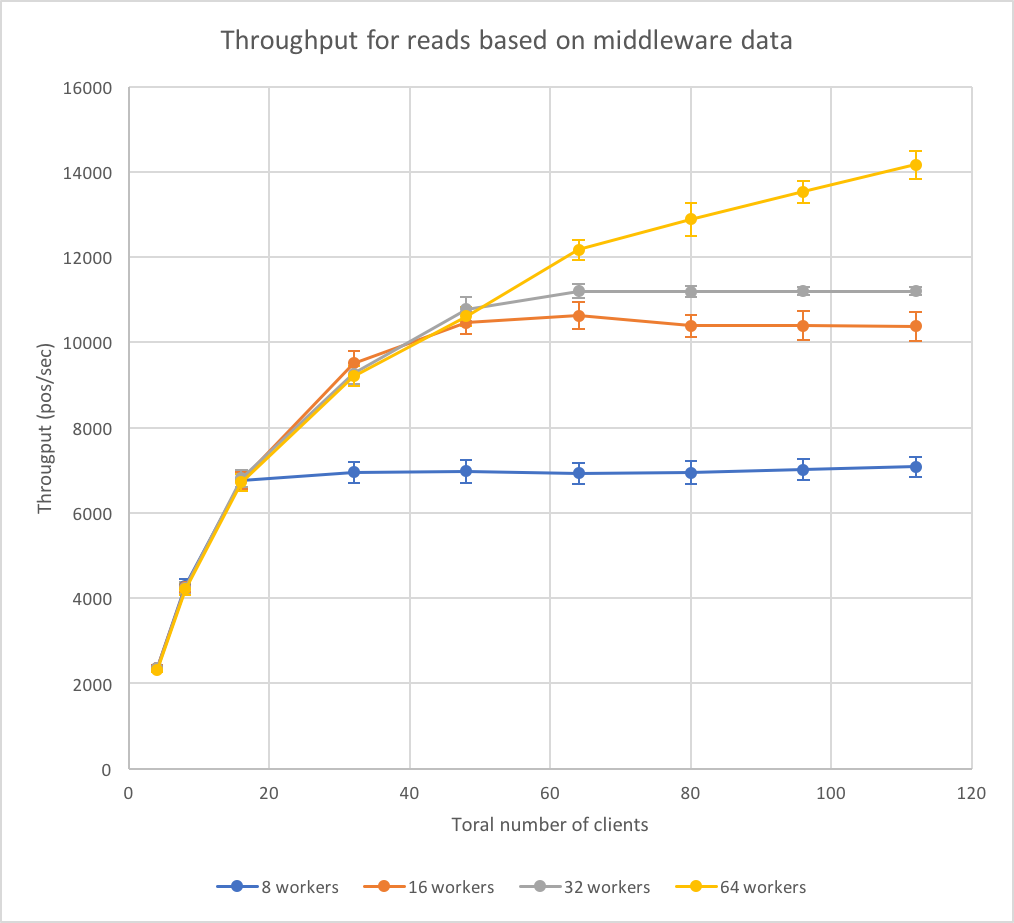
\includegraphics[width=\textwidth]{processing/graphics/bench_1mw_through-clients_read_mdat.png}
        \caption{Throughput as measured by the middleware reads}
        \label{png::bench_1mw_through-clients_read_mdat}
    \end{minipage}
\end{figure}

Similarly, the graphs displaying response time versus total number of clients for reads shown in figures \ref{png::bench_1mw_latency-clients_read_cdat} and \ref{png::bench_1mw_latency-clients_read_mdat} are very similar. Note that there is an initial offset of about one millisecond between the data provided by the middleware and the data provided by the client. This is due to network latencies. The response time measured in the middleware is measured from the moment a request is read from the server socket up to the point the response is sent back to the client. Hence it does not include the time spend in the network by both the request before arrival in the middleware and by the response before reaching the client. This adheres to the ping data gathered before the experiment which resulted in an average of around 0.8 millisecond network latencies between those specific client and middleware hosts\footnote{\mintinline{shell}{/logs/benchmark_1mw(2017-11-17_20h58)/mw_1_ping.log}}.

\begin{figure}[!h]
    \centering
    \begin{minipage}[b]{.45\textwidth}
        \centering
        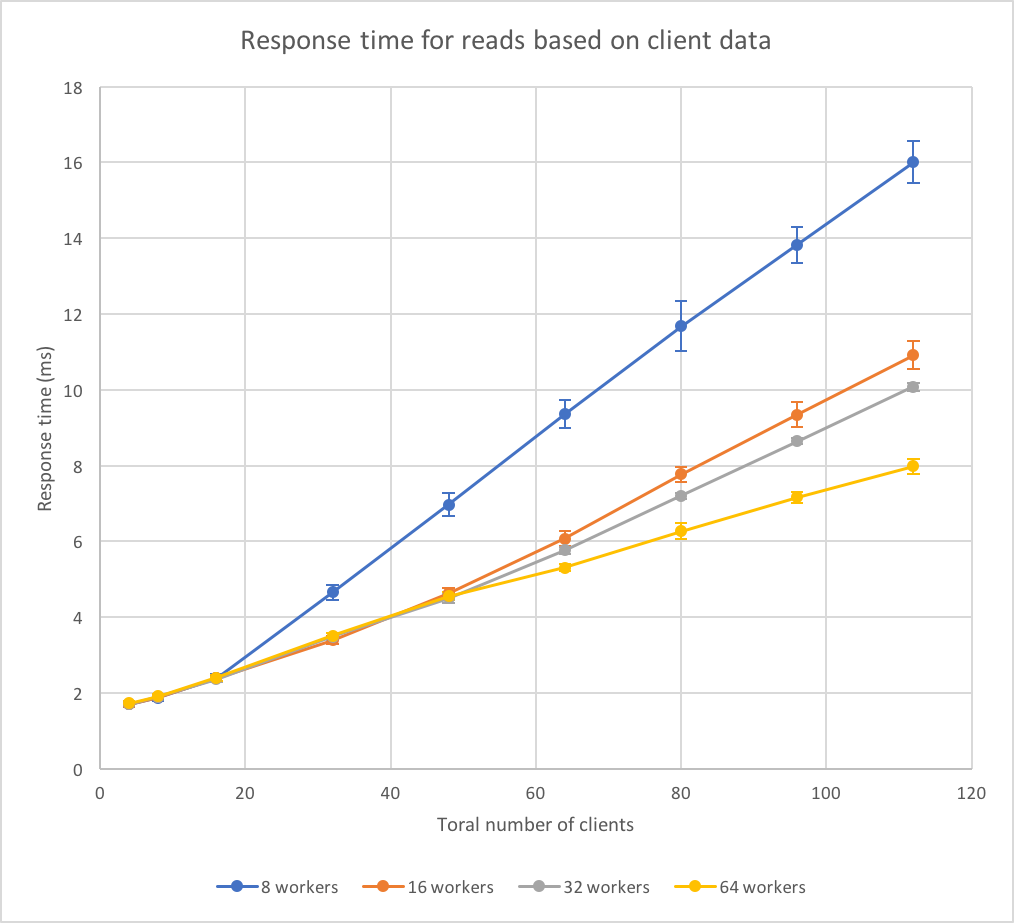
\includegraphics[width=\textwidth]{processing/graphics/bench_1mw_latency-clients_read_cdat.png}
        \caption{Response time as measured by the client machine for reads}
        \label{png::bench_1mw_latency-clients_read_cdat}
    \end{minipage}
    \qquad
    \begin{minipage}[b]{.45\textwidth}
        \centering
        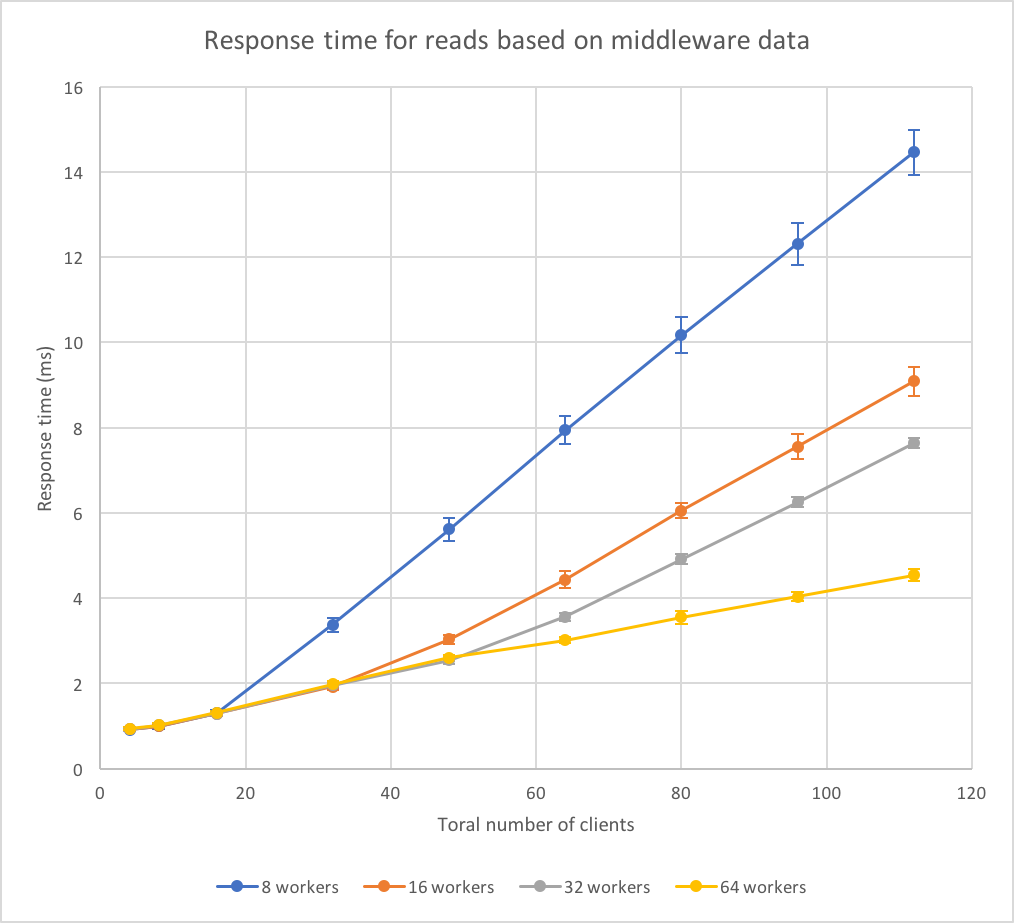
\includegraphics[width=\textwidth]{processing/graphics/bench_1mw_latency-clients_read_mdat.png}
        \caption{Response time as measured by the middleware for reads}
        \label{png::bench_1mw_latency-clients_read_mdat}
    \end{minipage}
\end{figure}

This kind of comparison between middleware and client data will not be included in future experiments. In the case of discrepancies between data aggregated by the middleware and the clients, this will be made explicit and explained. Hence no such comparison implicitly means that the data has no significant enough mismatches to require explanations.

\paragraph{8 workers}
In the case of 8 workers, the saturation is reached due to time taken to process a request, i.e. the time from the moment the request is dequeued to the time the response is sent back to the client. Note that the average time spent in the network between client and middleware (both when sending a request and receiving a response), is about one millisecond. Now note that the average time taken to process a single request when using 8 workers is also about one millisecond. Hence as long as less two times more clients than workers are sending requests, workers are efficient enough. This can easily be seen by considering that after a worker has completed a request for a client, it will take about 1 millisecond for another request from said client to arrive in the queue (due to network latencies), during which the worker can perform exactly one other request. Hence any number of clients superior to 16 ($2\times8$ workers) will not increase throughput as all workers will necessarily already be busy. A consequence of this is increased queue times and thus increased queue lengths (as seen in figure \ref{png::bench_1mw_ql_reads}). Therefore the middleware saturates at exactly 16 clients as can be seen in figure \ref{png::bench_1mw_latency-clients_read_mdat}. Of course this number depends on the environment the middleware is used in, as longer network latencies between middleware and clients will allow for more clients and vice-versa.\\
Beyond the client number for which the middleware saturates, server times also stabilise. This is due to the fact that memcached has to handle only as many request per second as the middleware can process. This becomes constant beyond the point of saturation, hence server times become constant as well (see figure \ref{png::bench_1mw_st_reads}).

\paragraph{16 workers}
For 16 workers, note that we encounter the same problem as for 8 workers. However, since we now have 16 workers working concurrently, this phenomenon only occurs with a number of clients superior to 32 ($2\times16$ workers). This is obvious when looking at figure \ref{png::bench_1mw_ql_reads}. As a direct consequence of this, server times stabilise beyond this point (see figure \ref{png::bench_1mw_st_reads}). The change is not as drastic as with 8 workers since the probability for slight changes in network latencies to result in a worker being idle increases with the number of workers. For example, due to a slight increase in network latency, more than 16 requests might be in the network between client and middleware, hence resulting in at least one worker being idle (by pigeonhole principle) if only 32 clients are used.

\paragraph{32 workers}
With this configuration, the network bandwidth becomes a problem once more. With 48 total clients, the memcached server has already nearly reached the network bandwidth limit. Again, this is can be computed manually as in section \ref{section::computation_reads}. As the throughput reaches levels close to 11k reads, the netowrk becomes the bottleneck.

\paragraph{64 workers}
Note that this data is skewed. Obviously, if for 32 workers the network was a bottleneck, increasing the number of worker should not increase throughput as indicated in figure \ref{png::bench_1mw_latency-clients_read_mdat}. The reason that throughput can increase beyond the levels without middleware is the following. The experiment was run on a rather large range of clients and all read repetitions were performed collectively. Hence during several hours the only operations sent to memcached were reads, this resulted in all cached data to be evicted while running the experiment with 64 workers. Table \ref{table::data_eviction} shows at what point exactly the data was evicted.

\begin{figure}[!h]
    \centering
    \begin{tabular}{|l|l|r|r|r|}
        \hline Ratio & Sharded & Workers & Client per thread & Hit/request ratio \\
        \hline 0:1 & false & 64 & 2 & 1 \\
        \hline 0:1 & false & 64 & 4 & 1 \\
        \hline 0:1 & false & 64 & 8 & 1 \\
        \hline 0:1 & false & 64 & 16 & 1 \\
        \hline 0:1 & false & 64 & 24 & 0.963838567 \\
        \hline 0:1 & false & 64 & 32 & 0 \\
        \hline 0:1 & false & 64 & 40 & 0 \\
        \hline 0:1 & false & 64 & 48 & 0 \\
        \hline 0:1 & false & 64 & 56 & 0 \\
        \hline
    \end{tabular}
    \caption{Data Eviction}
    \source{/processing/final/benchmark\_1mw/data.csv}
    \label{table::data_eviction}
\end{figure}

Therefore note that beyond 48 clients ($24\times2$ threads), memcached responses contain no more data, hence effectively removing the network bandwidth bound. In fact, average network sends per second are reduces from 11MB to slightly more than 8MB\footnote{\mintinline{shell}{processing/final/benchmark_1mw/dstat.xlsx!Sheet1}} per second even though throughput rises as indicated by figure \ref{png::bench_1mw_through-clients_mdat}. This also causes queue lengths to be much lower than normally as more requests can be handled by memcached. This can be seen in figure \ref{png::png::bench_1mw_ql_reads}. In the case of server times, they are first reduced due to less data having to be sent over the network, then increase beyond the level of 32 workers (figure \ref{png::bench_1mw_st_reads}) simply because much more requests have to be handled by memcached, hence increasing response time of the server. Normally, if the data eviction had not occurred, throughput with 64 workers should have behaved similarly to throughput with 32 workers.


\begin{figure}[!h]
    \centering
    \begin{minipage}[b]{.45\textwidth}
        \centering
        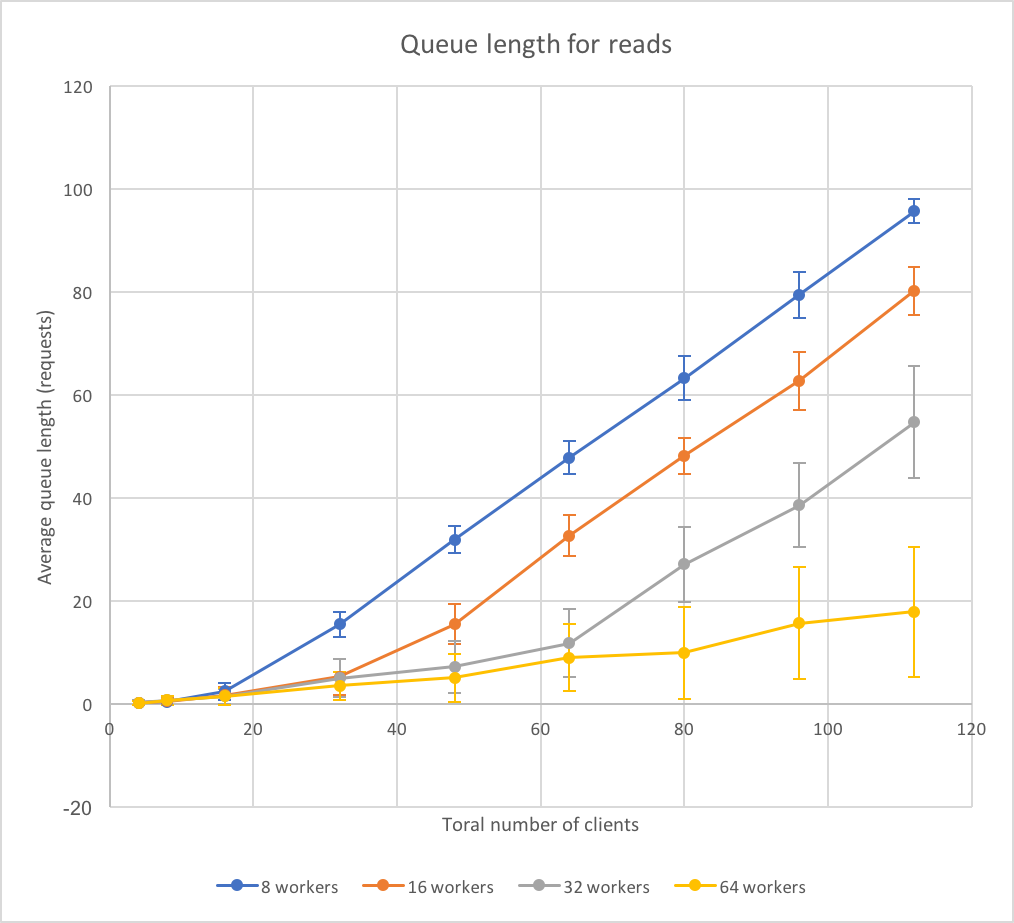
\includegraphics[width=\textwidth]{processing/graphics/bench_1mw_ql_reads.png}
        \caption{Queue length for reads}
        \label{png::bench_1mw_ql_reads}
    \end{minipage}
    \qquad
    \begin{minipage}[b]{.45\textwidth}
        \centering
        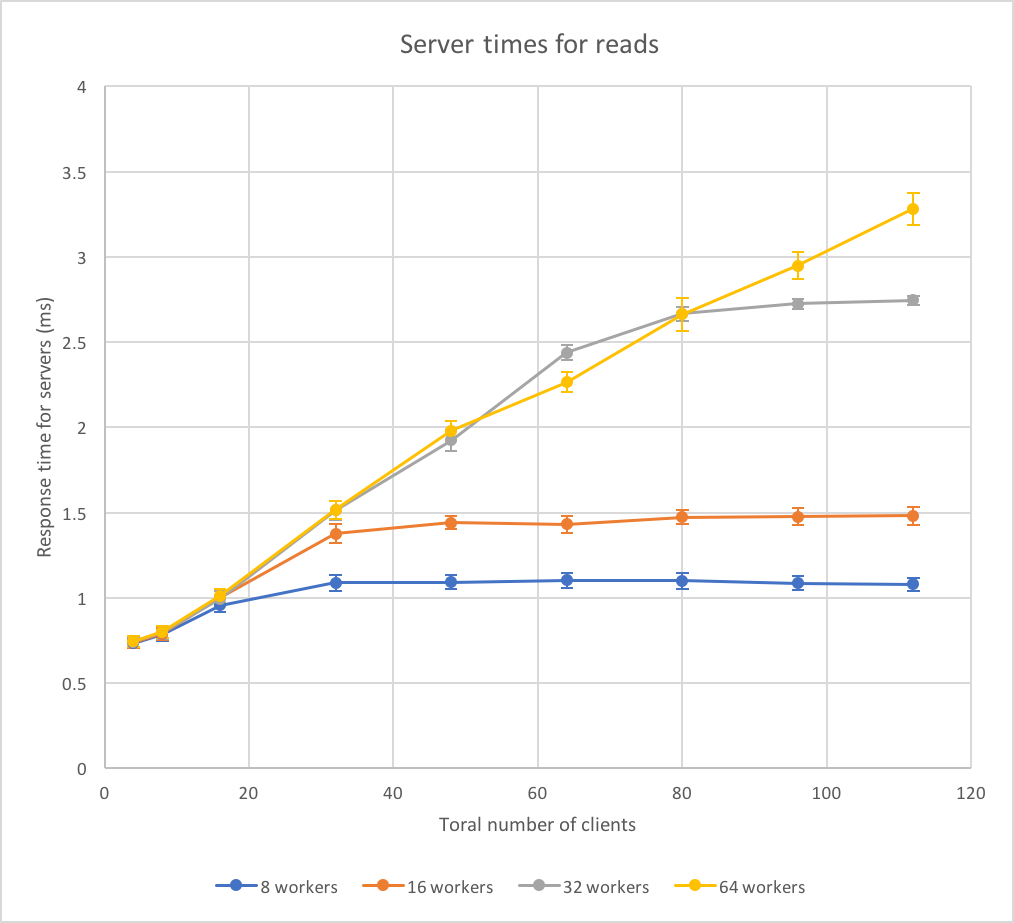
\includegraphics[width=\textwidth]{processing/graphics/bench_1mw_st_reads.png}
        \caption{Server time for reads}
        \label{png::bench_1mw_st_reads}
    \end{minipage}
\end{figure}


\subsubsection{Writes}
As discussed above, only middleware data will be shown in this section as it does not differ from client based data. Figure \ref{png::bench_1mw_through-clients_write_mdat} shows throughput as a function of number of clients for write operations. Similarly, figure \ref{png::bench_1mw_latency-clients_write_mdat} shows response time as a function of total client number for write operations based on middleware data.

\begin{figure}[!h]
    \centering
    \begin{minipage}[b]{.45\textwidth}
        \centering
        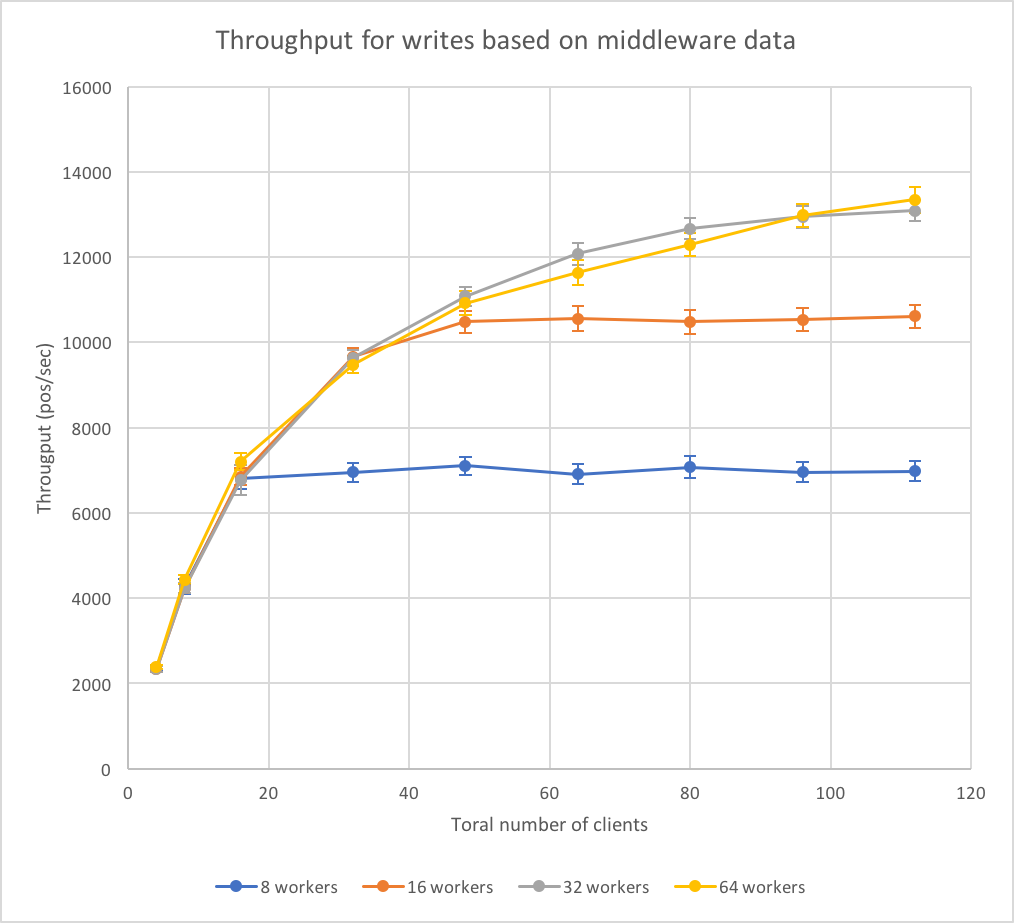
\includegraphics[width=\textwidth]{processing/graphics/bench_1mw_through-clients_write_mdat.png}
        \caption{Throughput as a function of clients for writes}
        \label{png::bench_1mw_through-clients_write_mdat}
    \end{minipage}
    \qquad
    \begin{minipage}[b]{.45\textwidth}
        \centering
        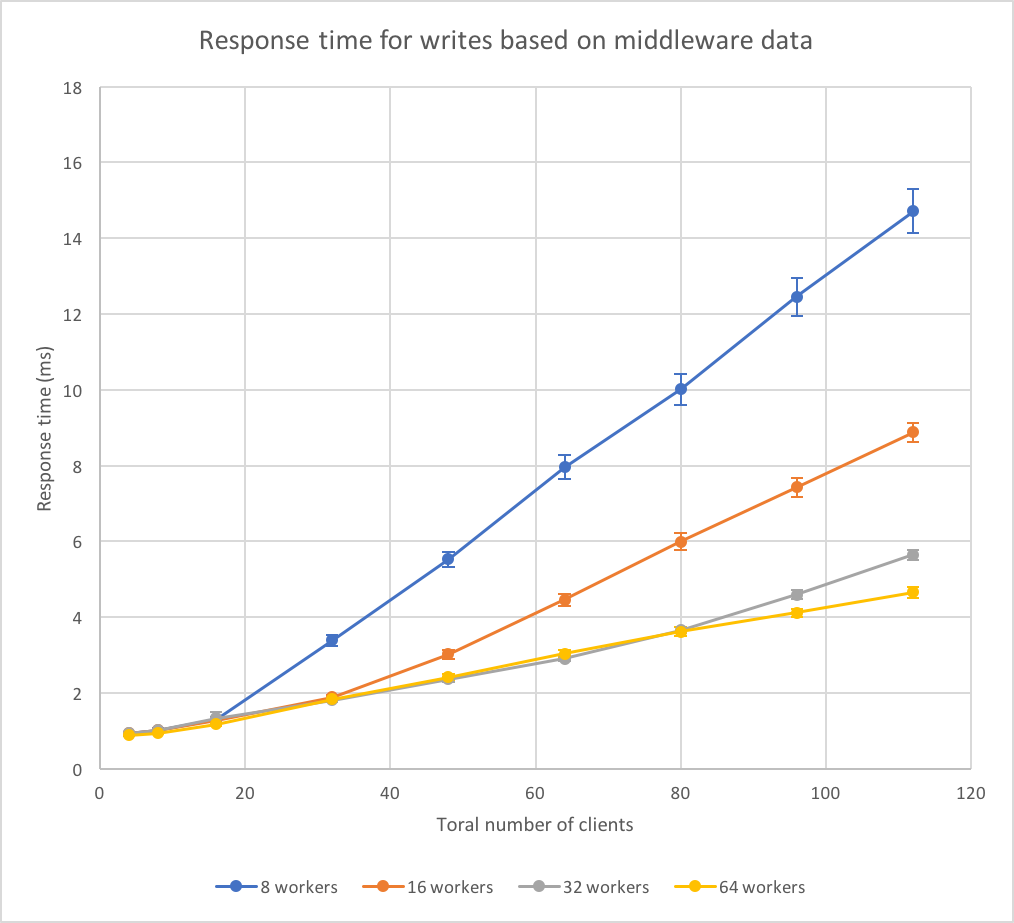
\includegraphics[width=\textwidth]{processing/graphics/bench_1mw_latency-clients_write_mdat.png}
        \caption{Response time as a function of clients for writes}
        \label{png::bench_1mw_latency-clients_write_mdat}
    \end{minipage}
\end{figure}

\paragraph{All worker counts}
With 8 workers, the same issue as for reads with 8 workers is encountered. One can clearly see in figure \ref{png::bench_1mw_through-clients_write_mdat} that past 16 clients the system is saturated. Unsurprisingly, as network latencies between client and middleware, and between middleware and server are similar to the ones for reads, the throughput attained when saturated is comparable. Note that the same problem is encountered for all worker configurations. The server response time increases as throughput increases (see figure \ref{png::bench_1mw_st_writes}), just as presented in the server baseline and shown in figure \ref{png::bench_memcached_latency-clients}. This causes increasing processing times in the middleware thus reducing the speed up by doubling worker counts. Moreover, the network latencies between client and middleware increase in parallel to this hence preserving the ratio of about 2 clients per worker before reaching saturation. For example, figure \ref{png::bench_1mw_netlat_st_64writes} shows the change in server times and network latencies between middleware and clients. Note that the network latencies are computed by taking the difference in response time measured by the middleware and the response time measured by the client machine. The increase in this latency is likely due to the fact that the net-thread in the middleware cannot read from requests from the network fast enough. Thus, when a large amount of requests arrive in very short time windows, some of the request need to wait a relatively long time before being read by the net thread and added to the queue.

\begin{figure}[!h]
    \centering
    \begin{minipage}[b]{.45\textwidth}
        \centering
        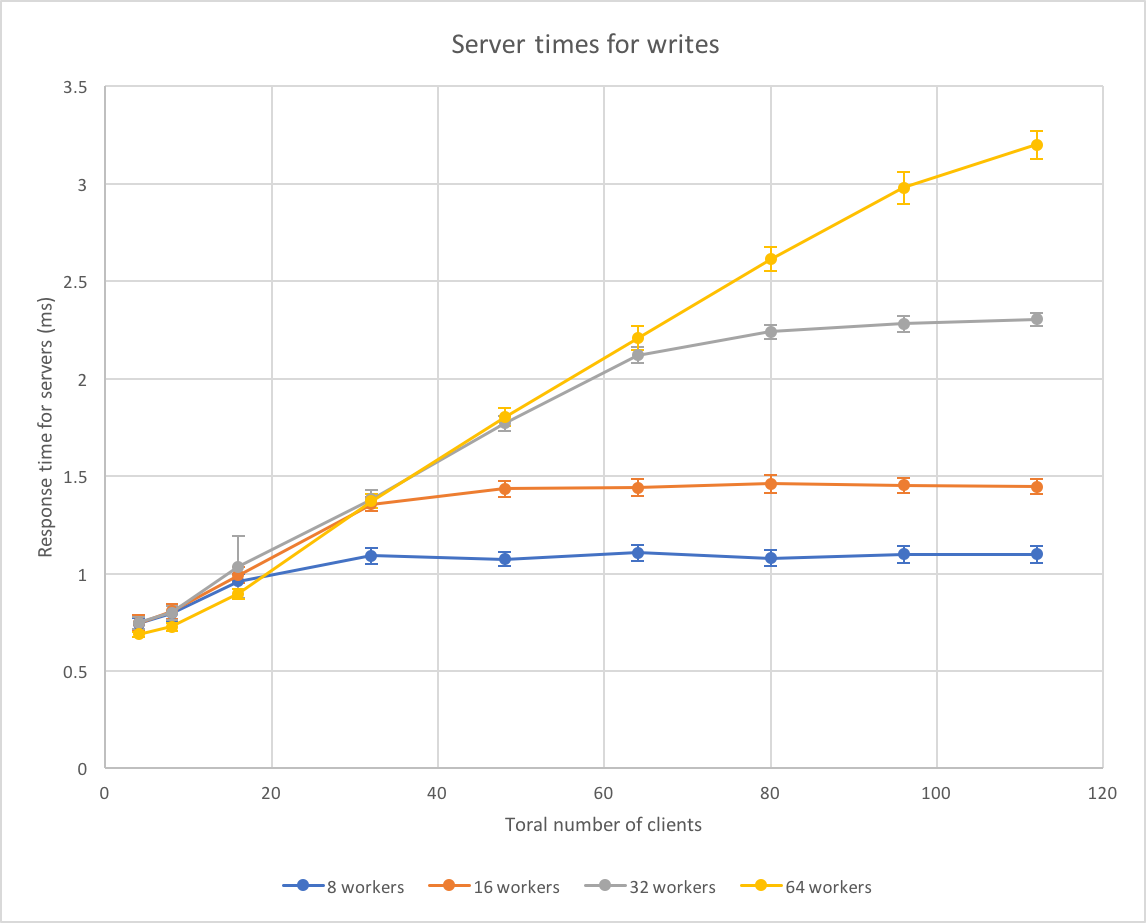
\includegraphics[width=\textwidth]{processing/graphics/bench_1mw_st_writes.png}
        \caption{Server time (time in network + time in server) for writes}
        \label{png::bench_1mw_st_writes}
    \end{minipage}
    \qquad
    \begin{minipage}[b]{.45\textwidth}
        \centering
        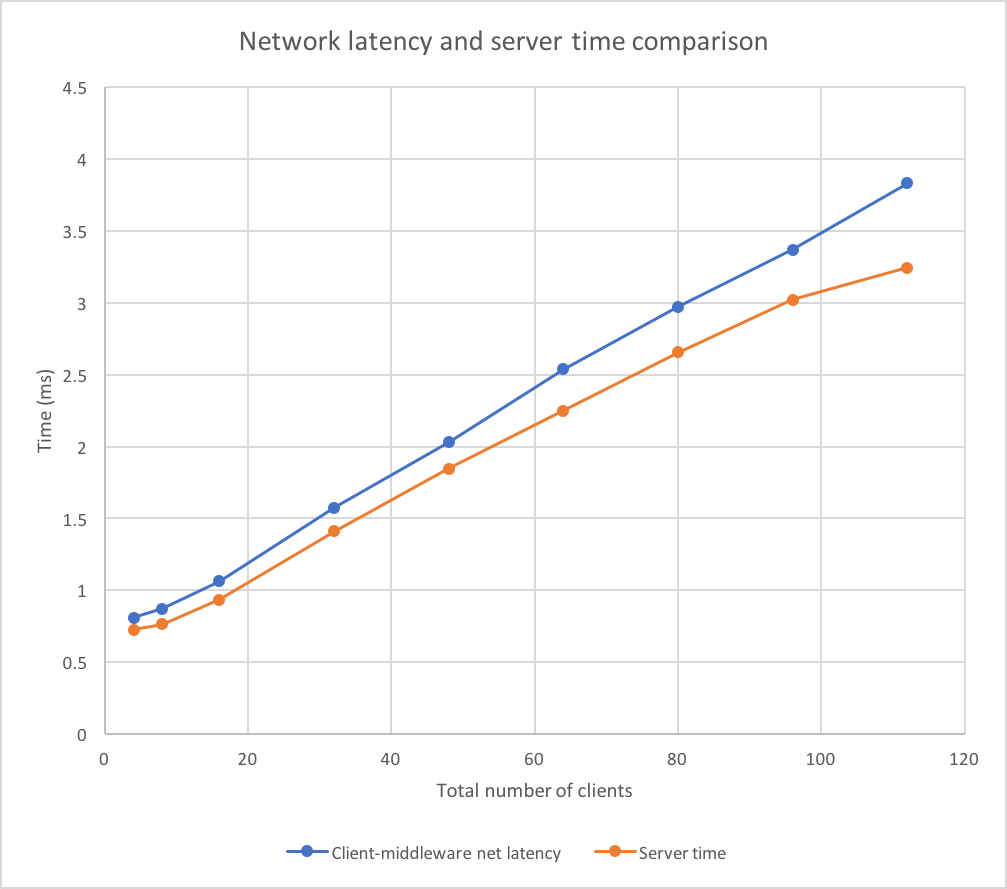
\includegraphics[width=\textwidth]{processing/graphics/bench_1mw_netlat_st_64writes.png}
        \caption{Network latency and server time for writes with 64 workers}
        \label{png::bench_1mw_netlat_st_64writes}
    \end{minipage}
\end{figure}



\subsection{Two middlewares}
\subsubsection{Reads}
Figures \ref{png::bench_2mw_through-clients_reads} and \ref{png::bench_2mw_latency-clients_reads} show the throughput and response time as a function of client count for reads. Figure shows the total throughput across both middlewares.
Once again, data was evicted while the experiment was running. This causes throughput with 64 workers to increase above levels with other configurations. This is again due to the fact that the network is a bottlenecks for 8, 16, and 32 workers. The server cannot upload data fast enough to handle more requests. However, as data gets evicted, requests require less data to be uploaded by the server (due to empty responses), hence allowing more requests to be performed per second. Average hit to request ratio drops from 79.6\% to 8.7\%\footnote{\mintinline{shell}{/processing/final/benchmark_2mw/benchmark_2mw.xlsx}} between 16 and 24 client runs with 64 workers. This results in only around 2.6MB\footnote{\mintinline{shell}{/processing/final/benchmark_2mw/dstat.csv}} of data per second uploaded by the server. Therefore, higher throughputs are possible.

\begin{figure}[!h]
    \centering
    \begin{minipage}[b]{.45\textwidth}
        \centering
        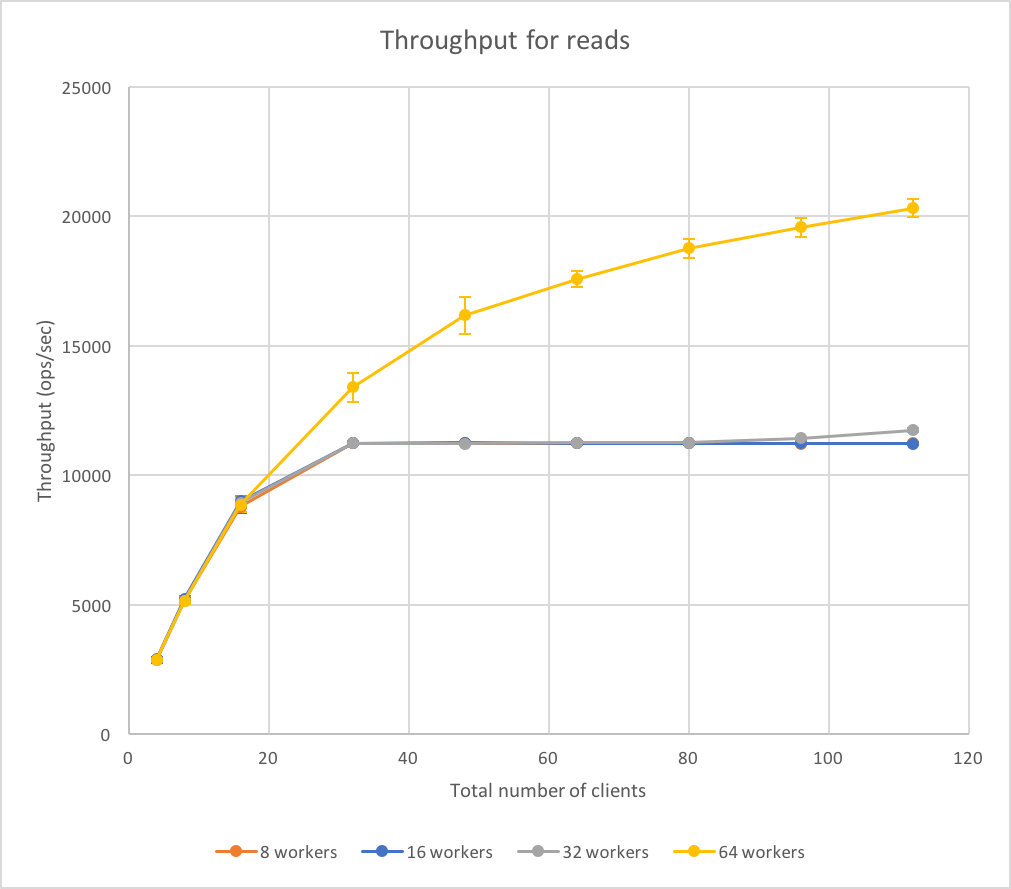
\includegraphics[width=\textwidth]{processing/graphics/bench_2mw_through-clients_reads.png}
        \caption{Throughput as a function of clients for reads}
        \label{png::bench_2mw_through-clients_reads}
    \end{minipage}
    \qquad
    \begin{minipage}[b]{.45\textwidth}
        \centering
        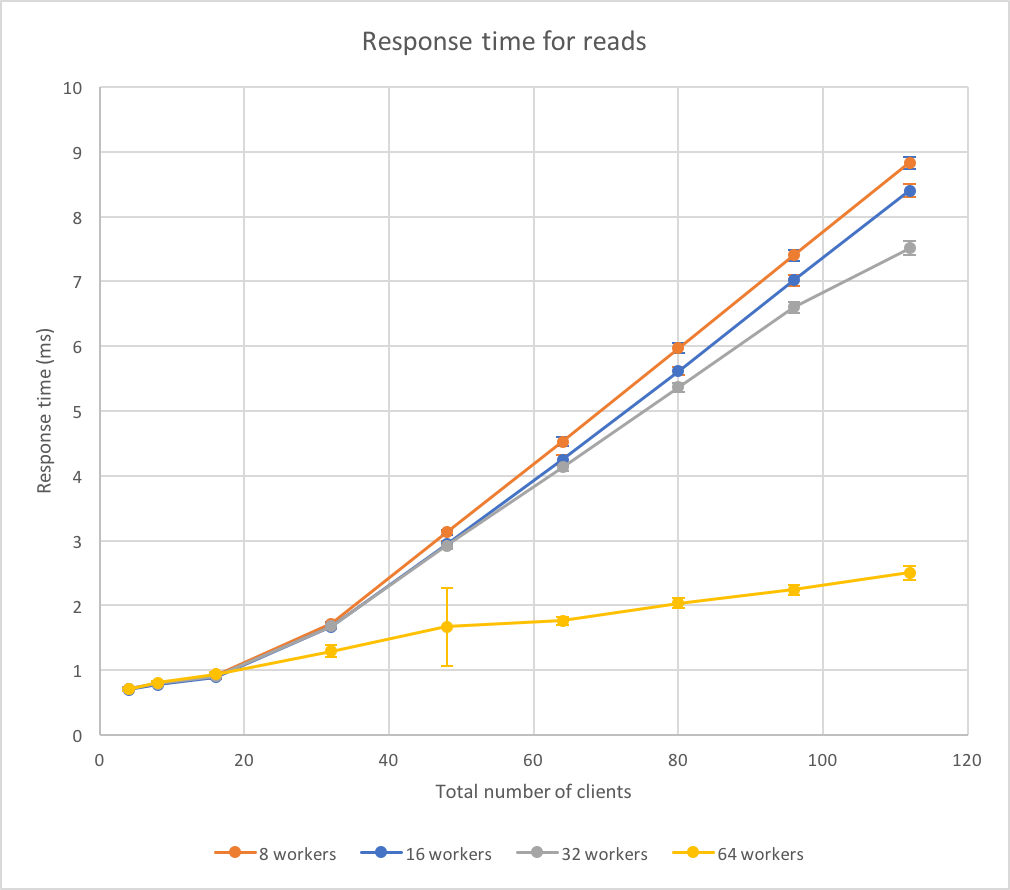
\includegraphics[width=\textwidth]{processing/graphics/bench_2mw_latency-clients_reads.png}
        \caption{Response time as a function of clients for reads}
        \label{png::bench_2mw_latency-clients_reads}
    \end{minipage}
\end{figure}

\subsubsection{Writes}
Figure \ref{png::bench_2mw_through-clients_writes} clearly has a dent with 16 workers. This is caused by a sudden increase in network latencies between the middleware and the memcached server. When testing with 16 workers, the last repetition with 32 clients per threads and the first repetition with 40 clients per thread experienced server times more than 2 times higher than normal\footnote{\mintinline{shell}{/processing/processed/benchmark_2mw/ratio_1:0/sharded_false/workers_16/clients_32/mws.csv}}. The deviation in throughput and response time between repetitions hence increased thirtyfold between 24 and 32 clients\footnote{\mintinline{shell}{/processing/final/benchmark_2mw/data.csv}}. It actually reached normal levels again only when testing with 56 clients per thread.

The increase in network latencies between middlewares and server is likely caused by a short burst in network traffic on Microsoft Azure resulting in higher network latencies between middlewares and server. Hence processing requests takes more time resulting in lower throughput and higher response times.

\begin{figure}[!h]
    \centering
    \begin{minipage}[b]{.45\textwidth}
        \centering
        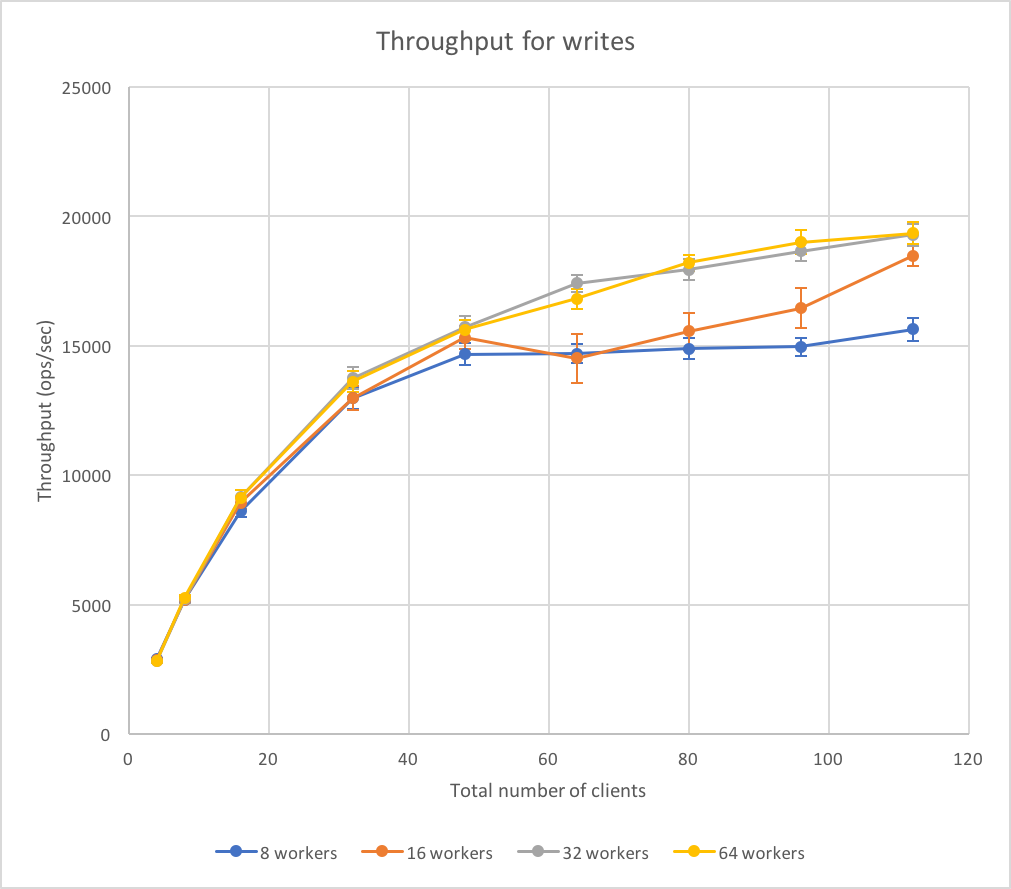
\includegraphics[width=\textwidth]{processing/graphics/bench_2mw_through-clients_writes.png}
        \caption{Throughput as a function of clients for writes}
        \label{png::bench_2mw_through-clients_writes}
    \end{minipage}
    \qquad
    \begin{minipage}[b]{.45\textwidth}
        \centering
        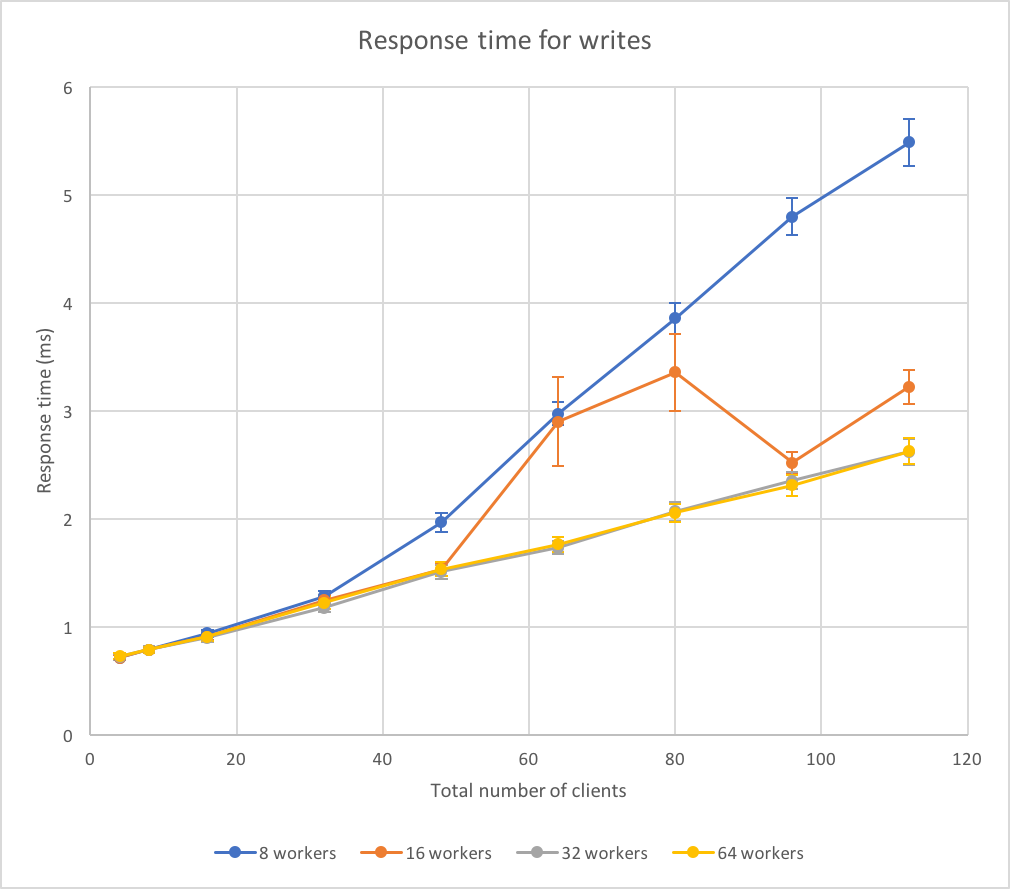
\includegraphics[width=\textwidth]{processing/graphics/bench_2mw_latency-clients_writes.png}
        \caption{Response time as a function of clients for writes}
        \label{png::bench_2mw_latency-clients_writes}
    \end{minipage}
\end{figure}

The bottleneck with these configurations is the net-thread as for reads. Figure \ref{png::bench_2mw_netlat_writes} shows the difference in response time measured by the client and the middlewares. The dent for 16 workers is due to the fact that middleware 2 had very low server times\footnote{\mintinline{shell}{/processing/processed/benchmark_2mw/ratio_1:0/sharded_false/workers_16/clients_48/mws.csv}}. This lead to reduced response times for said middleware, decreasing the average response time of the middleware and increasing the difference in measured response times between client and middlewares.

In all cases (8, 16, 32 and 64 workers), the response time difference between client and middlewares increases steadily. This suggests that the net-thread cannot read the requests fast enough to put them on the queue, hence creating latencies between client and middlewares. The reason the increase is less significant for 8 clients is that response time increases much more than for 32 or 64 clients. Hence less requests are in the network between client and middlewares at any given time, thus making the net-thread reading less of a bottleneck.

\begin{figure}[!h]
    \centering
    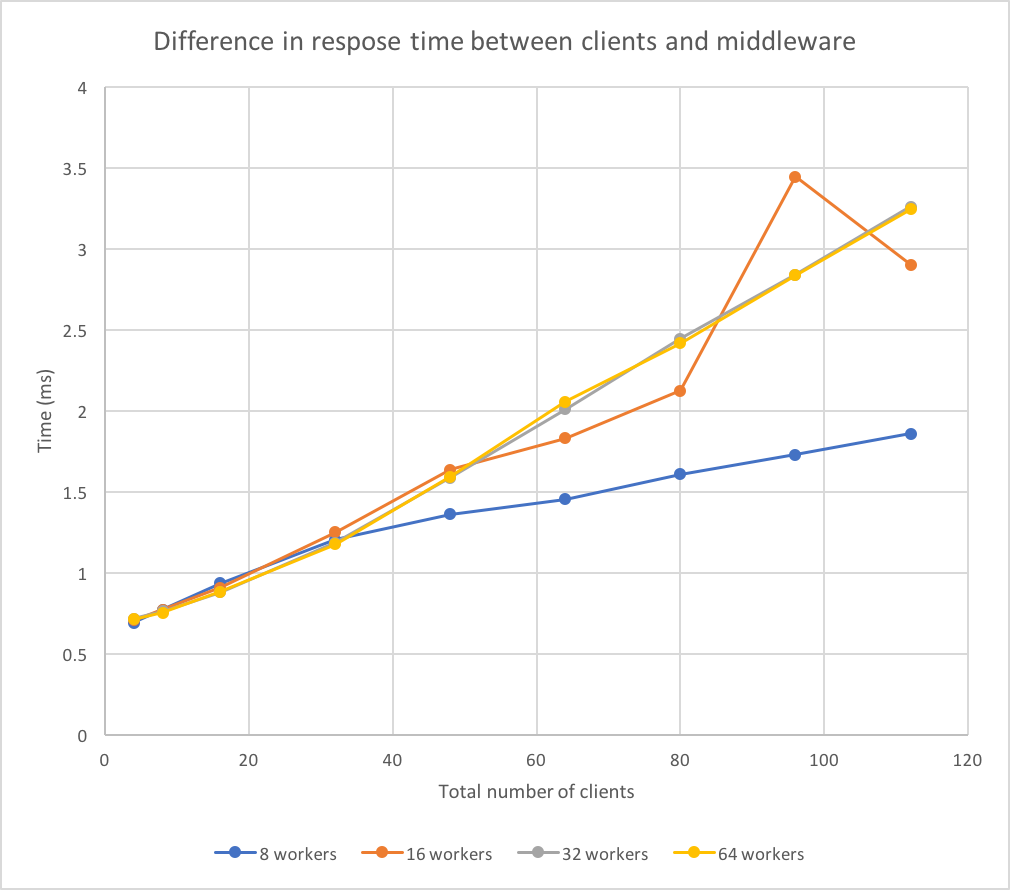
\includegraphics[width=.45\textwidth]{processing/graphics/bench_2mw_netlat_writes.png}
    \caption{Difference in response time between clients and middleware for writes}
    \label{png::bench_2mw_netlat_writes}
\end{figure}

\subsection{Summary}
Tables \ref{table::max_through_section_3_1mw} and \ref{table::max_through_section_3_2mw} show the maximum throughputs and the corresponding response times as measured by middlewares and the client machine in this section. Note that for reads, the maximum throughputs were chosen irrespective of miss rates, hence the figures are much higher than could be expected with low miss rates. If hit rates were taken into account, the maximum throughput for reads would be comparable to the one in figure \ref{table::max_through_section_2} for a single server. This would be the case for both a system with a single middleware, and one with two middlewares. However, due to high miss rates, the server does not require much data to be sent back to the middleware(s). Therefore the network bandwidth no longer creates a bottleneck, allowing to obtain higher throughput.

Moreover, the system with two middlewares performs nearly twice as well as the system with a single one. Response times are reduced by about two milliseconds both as measured by middlewares and by clients. Average time spent in queue is also reduced considerably. This directly follows from the fact that less requests have to be handled \textit{per middleware} in a system with more middlewares.


\begin{figure}
    \centering
	\begin{tabular}{|l|p{2cm}|p{2cm}|p{2cm}|p{2cm}|}
		\hline                                & Throughput & Response time & Average time in queue & Miss rate \\
		\hline Reads: Measured on middleware  &     14 162 &          4.54 &                  1.21 &     100\% \\
		\hline Reads: Measured on clients     &     14 049 &          7.98 & n/a                   &     100\% \\
		\hline Writes: Measured on middleware &     13 343 &          4.66 &                  1.41 & n/a       \\
		\hline Writes: Measured on clients    &     13 208 &          8.49 & n/a                   & n/a       \\
		\hline
	\end{tabular}
    \caption{Maximum throughput for one middleware}
    \label{table::max_through_section_3_1mw}
\end{figure}

\begin{figure}
    \centering
	\begin{tabular}{|l|p{2cm}|p{2cm}|p{2cm}|p{2cm}|}
		\hline                                & Throughput & Response time & Average time in queue & Miss rate \\
		\hline Reads: Measured on middleware  &     20 303 &          2.50 &                  0.47 &     100\% \\
		\hline Reads: Measured on clients     &     20 113 &          5.60 & n/a                   &     100\% \\
		\hline Writes: Measured on middleware &     19 349 &          2.63 &                  0.46 & n/a       \\
		\hline Writes: Measured on clients    &     19 205 &          5.87 & n/a                   & n/a       \\
		\hline
	\end{tabular}
    \caption{Maximum throughput for two middlewares}
    \label{table::max_through_section_3_2mw}
\end{figure}

\newpage

\section{Throughput of writes}
During this experiment, three load generating virtual machines running two instances of memtier each are connected to two middlewares. Each instance of memtier runs on a single thread. The two middlewares are hosted on different virtual machines and are connected to three backend memcached servers.

As the title indicates, the experiment is run on write-only workloads with a range of different client numbers. Moreover, the number of worker threads is changed in the middlewares, same as in the last section.

As shown in figure \ref{png::throughput_writes_through-clients}, each increase in workers increases the overall performance of the system. The middlewares already saturate at 24 clients when running with 8 workers. This follows from the time taken for servers to respond to the middlewares. Note that the base time spent waiting for servers is much higher when using three backend servers compared to a single memcached server. This is caused by the fact that if one of the three servers is very slow (due to network latencies or CPU bounds), the worker is idle waiting for a response. Moreover, much more data has to be sent over the network since \textit{all} data from \mintinline{java}{set} request is sent to all servers (not just parts such as in sharded \mintinline{java}{mutliget} requests). Hence it requires the middlewares to send exactly three times as much data as with a single server. This results in longer response times and, by operational laws, in lower throughput.

\begin{figure}[!h]
    \centering
    \begin{minipage}[b]{.45\textwidth}
        \centering
        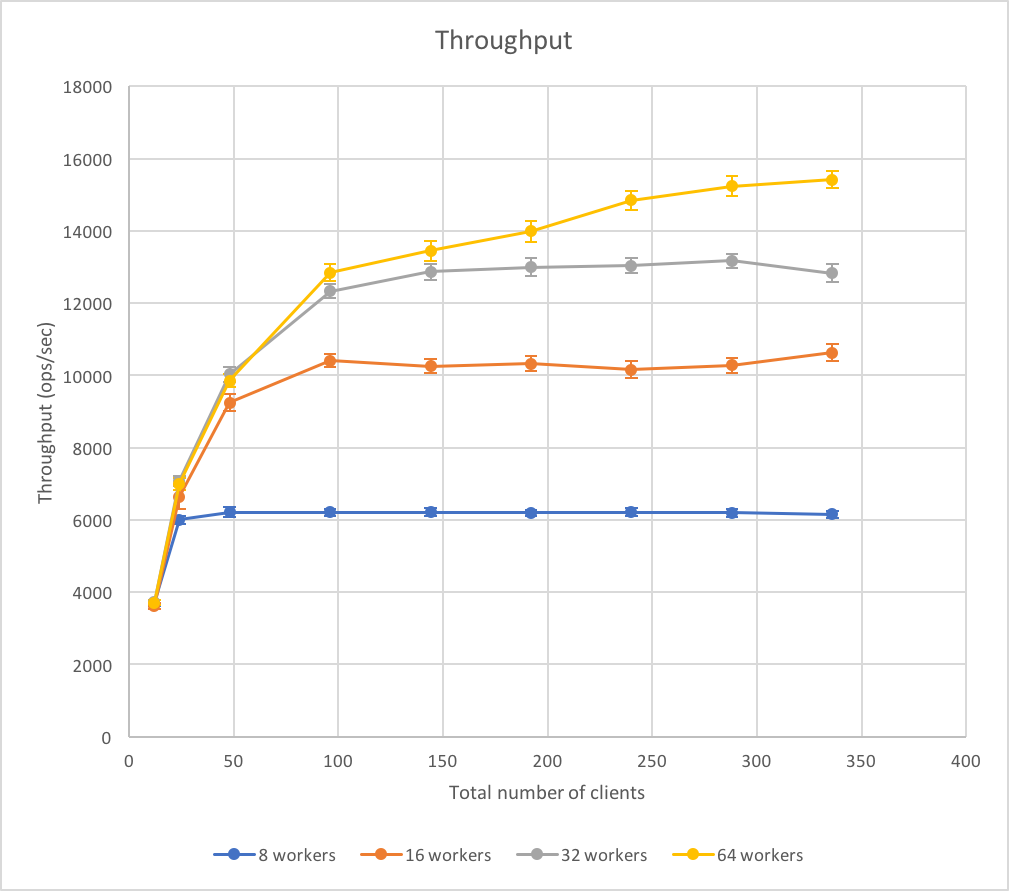
\includegraphics[width=\textwidth]{processing/graphics/throughput_writes_through-clients.png}
        \caption{Throughput as a function of clients}
        \label{png::throughput_writes_through-clients}
    \end{minipage}
    \qquad
    \begin{minipage}[b]{.45\textwidth}
        \centering
        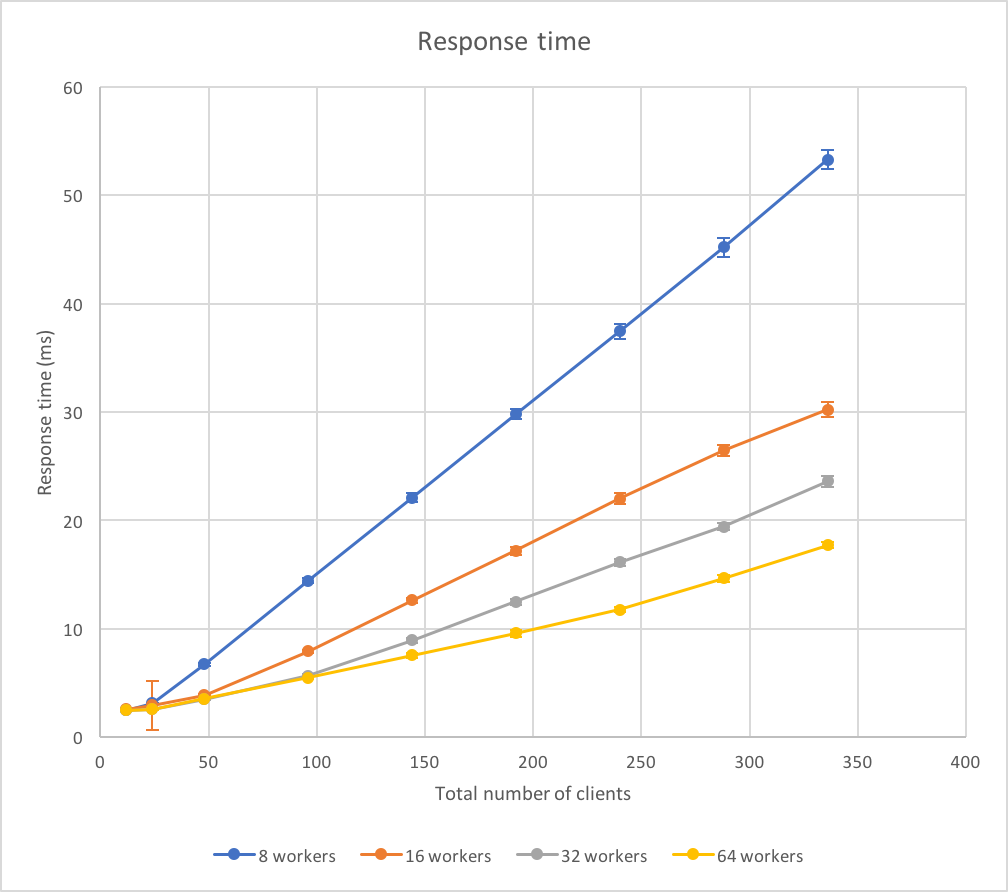
\includegraphics[width=\textwidth]{processing/graphics/throughput_writes_latency-clients.png}
        \caption{Response time as a function of clients}
        \label{png::throughput_writes_latency-clients}
    \end{minipage}
\end{figure}

Note that the drop in throughput compared to single server systems is very significant. In figure \ref{png::bench_2mw_through-clients_writes}, one can see throughput levels above 10 thousand requests per second. In the current case, 24 total clients results in barely over 6 thousand requests per second (figure \ref{png::throughput_writes_through-clients}). When comparing the time spend processing a request for both these system setups, one can see that the actual time spent processing (without time spent waiting for servers) is about the same at 0.03 milliseconds\footnote{\mintinline{shell}{/processing/final/*/data.csv}}. However, the time spent waiting for servers changes considerably. With three servers, this is more constant as clients increase, only ranging from 2.38 to 2.55 milliseconds over the entire range of clients\footnote{\mintinline{shell}{/processing/final/throughput_writes/data.csv}}. With a single server, the server time is less constant but much lower, increasing from 0.63 milliseconds for 4 clients to 1.41 milliseconds for 112 clients\footnote{\mintinline{shell}{/processing/final/benchmark_2mw/data.csv}}. This stability in server time is only present for low worker count though. When running the middlewares with more workers, server times increase with client count as seen in figure \ref{png::throughput_writes_st}.

This general offset in server times when using three backend servers results in earlier saturation of the middlewares. Taking the configuration with 8 workers as an example once more, the system with a single memcached server saturates at 48 total clients (24 per middleware) as seen in figure \ref{png::bench_2mw_through-clients_writes}. In the case considered during this experiment, the system already saturates at 24 total clients (12 per middleware) as seen in figure \ref{png::throughput_writes_through-clients}.

For all worker configurations, the bottleneck is the service time of the servers. Due to the increase in server time, doubling the number of workers does not quite double the throughput at saturation level. However, note that in the case of switching from 8 workers to 16, the server time does not increase considerably, hence allowing for nearly twice the throughput at saturated levels (from about 6 thousand to about 10 thousand requests per second).

Figure \ref{png::throughput_writes_ql} shows how queue length varies with increases in client counts. On this graph, one can distinctly see how an increase in the number of clients on a saturated system simply increases the queue length linearly. For 8 workers, this happens beyond 24 clients; for 16 workers, beyond 48 clients; for 32 workers, beyond 96 clients; and for 64 workers at around 192 clients.

\begin{figure}[!h]
    \centering
    \begin{minipage}[b]{.45\textwidth}
        \centering
        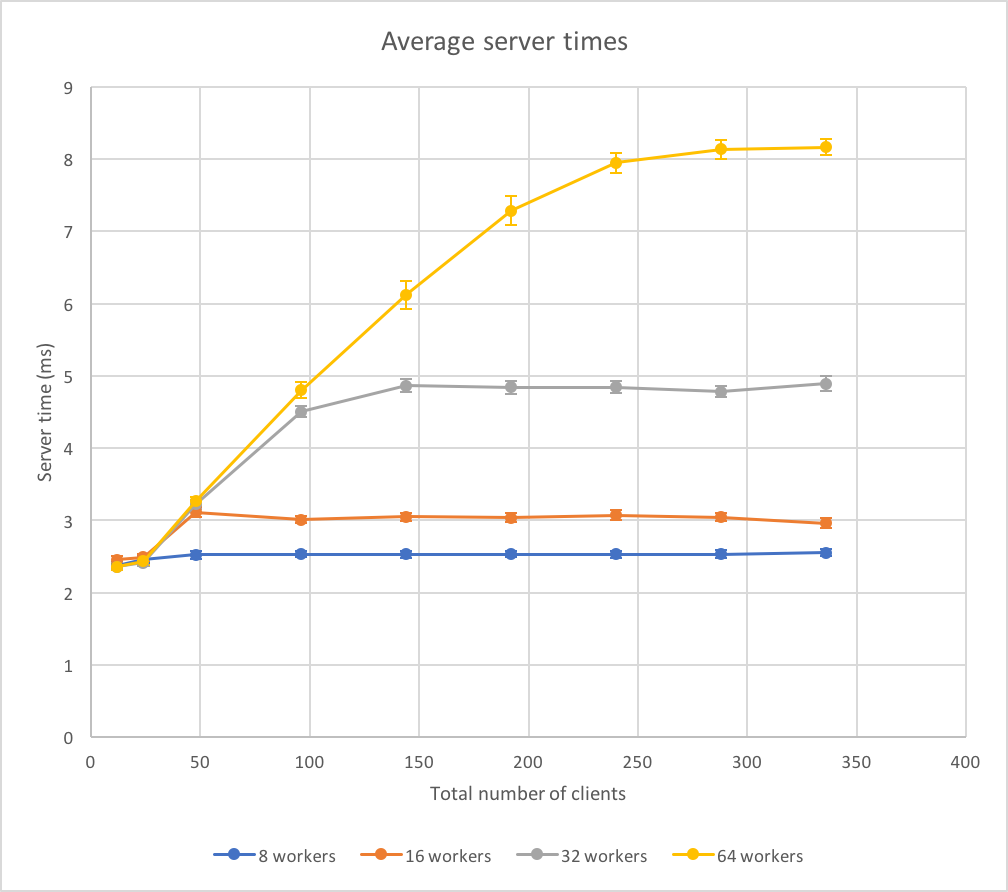
\includegraphics[width=\textwidth]{processing/graphics/throughput_writes_st.png}
        \caption{Average server times as a function of total number of clients}
        \label{png::throughput_writes_st}
    \end{minipage}
    \qquad
    \begin{minipage}[b]{.45\textwidth}
        \centering
        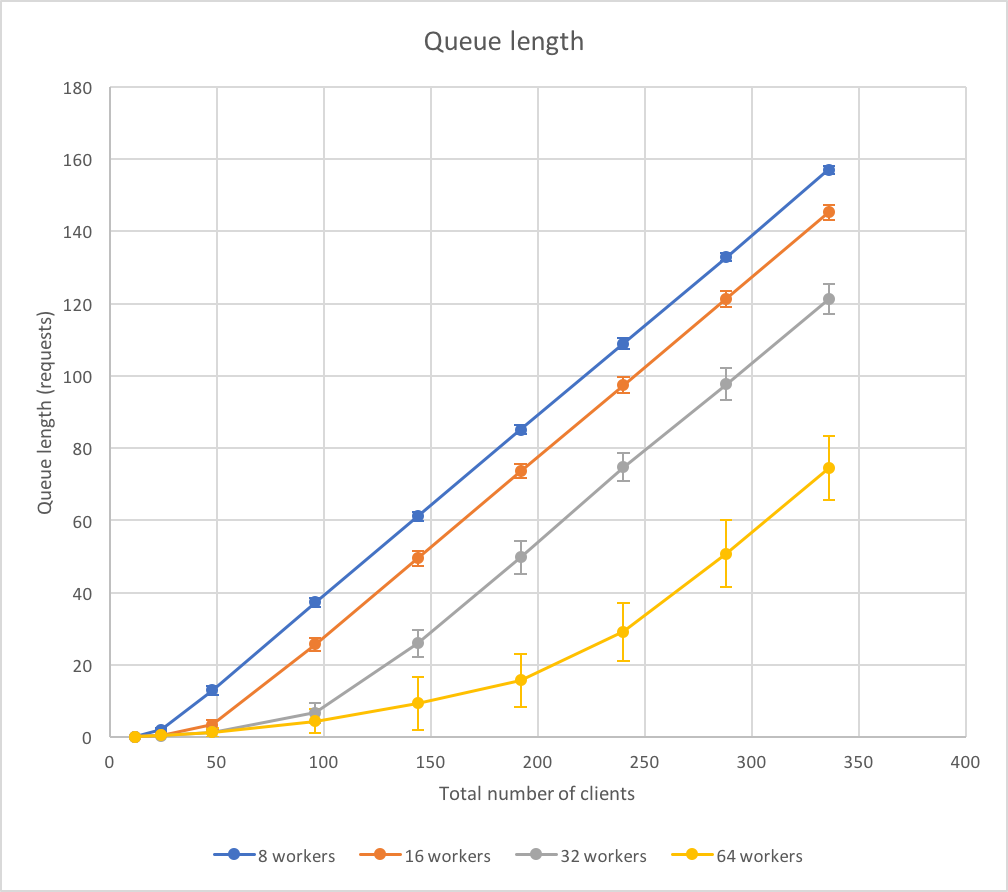
\includegraphics[width=\textwidth]{processing/graphics/throughput_writes_ql.png}
        \caption{Queue length as a function of total number of clients}
        \label{png::throughput_writes_ql}
    \end{minipage}
\end{figure}

Table \ref{table::max_through_section_4} shows maximum throughput as measured by middleware and clients as well as more information at that level of throughput. Note that for the throughput derived from the middleware response time, the following formula is used:
$$
X = \frac{N}{R + Z}
$$
The think time used ($Z$) is 0 as technically it would be equal to the time taken to send a response back to the client and the client sending a request back to the middleware. However, this would mean that $R + Z$, with $R$ being the response time measured by the middleware, is equal to the response time measured by the client. As this obviously follows operational laws, it would be redundant to compute this.

\begin{figure}[!h]
    \centering
	\begin{tabular}{|l|p{1.5cm}|p{1.5cm}|p{1.5cm}|p{1.5cm}|}
		\hline                                            &   WT=8 &   WT=16 &   WT=32 &   WT=64 \\
		\hline Throughput (Middleware)                    &   6218 &  10 624 &  13 175 &  15 421 \\
		\hline Throughput (Derived from MW response time) &   6412 &  11 115 &  14 814 &  18 971 \\
		\hline Throughput (Client)                        &   6164 &  10 529 &  13 060 &  15 261 \\
		\hline Average time in queue                      &  34.88 &   27.24 &   14.62 &    9.50 \\
		\hline Average length of queue                    &  108.9 &   145.3 &    97.7 &    74.5 \\
		\hline Average time waiting for memcached         &   2.53 &    2.96 &    4.78 &    8.17 \\
		\hline
	\end{tabular}
    \caption{Maximum throughput for the full system}
    \label{table::max_through_section_4}
\end{figure}

The figures displayed in table \ref{table::max_through_section_4} clearly show that 64 workers provide the highest throughput and lowest response time. Moreover, the gap between measured throughputs and throughputs computed with the interactive law increases this the number of workers. This is caused by the increase in difference between the response time measured by clients and the response time measured by the middlewares. That difference increases due to the fact that the net-thread has less available resources to read from the network as more worker threads read and write from network, hence creating a queue in the socket server. However, this is not a bottleneck as average queue lengths are still quite high. This would only become a problem is workers were able to process requests faster than the net-thread can read requests from the socket. However, this is by far not the case due to the time spent waiting for server responses.


\end{document}
